\documentclass{beamer}
\usepackage{graphicx}
\usepackage{tikz}
\usetikzlibrary{shapes,arrows}
\usepackage{tikz}
%\usecolortheme{seahorse}
  \setbeamertemplate{footline}[page number]
\usepackage{multirow}
\setbeamertemplate{navigation symbols}{}
\setbeamertemplate{frametitle}[default][center]
\setbeamerfont{frametitle}{shape=\scshape}
\usepackage{color}

\usepackage{csquotes}

\usepackage{xcolor}

\usepackage[flushleft]{threeparttable}

{\title{\textsc{Econ 352 - Search and Unemployment} \\ \tiny (See Williamson Ch. 6)}
\author{Trevor S. Gallen}
\date{}
\begin{document}
\renewcommand*{\inserttotalframenumber}{\pageref{lastframe}}


\setbeamertemplate{caption}{\raggedright\insertcaption\par}

\begin{frame}
\titlepage
\end{frame}

\begin{frame}
\frametitle[alignment=center]{Introduction}
\begin{itemize}
\item We built up the ``frictionless" (except taxes!) model of labor supply
\bigskip
\item This model does not please many, and yields challenges  
\bigskip
\item Why is there unemployment?  We'll build a model to think about it.
\bigskip
\item Important note: we will start talking about something some find dry:  firms and workers searching to fill jobs/vacancies and bargaining over wage.  \emph{if you find this boring}, please note that you can replace this with a male/female dating market! (more assumptions needed for homosexual dating market, feel free to ask when it comes up!)
\end{itemize}
\end{frame}

\begin{frame}
\frametitle[alignment=center]{Labor Market Facts}
\begin{itemize}
\item Let's review some of the facts and concepts.
\bigskip
\item Let $N$ be the working age population, $\mathcal{Q}$ be the labor force (employed+unemployed), and $U$ be the number of unemployed.  Then we define:
$$\text{unemployment rate}=\frac{U}{\mathcal{Q}}$$
$$\text{participation rate}=\frac{U}{\mathcal{N}}$$
$$\text{employment/population ratio}=\frac{\mathcal{Q}-U}{\mathcal{N}}$$
\bigskip
\item Let's look at the data first!
\end{itemize}
\end{frame}

\begin{frame}
\frametitle[alignment=center]{Unemployment Rate in the US}Figures
\begin{figure}
\centering
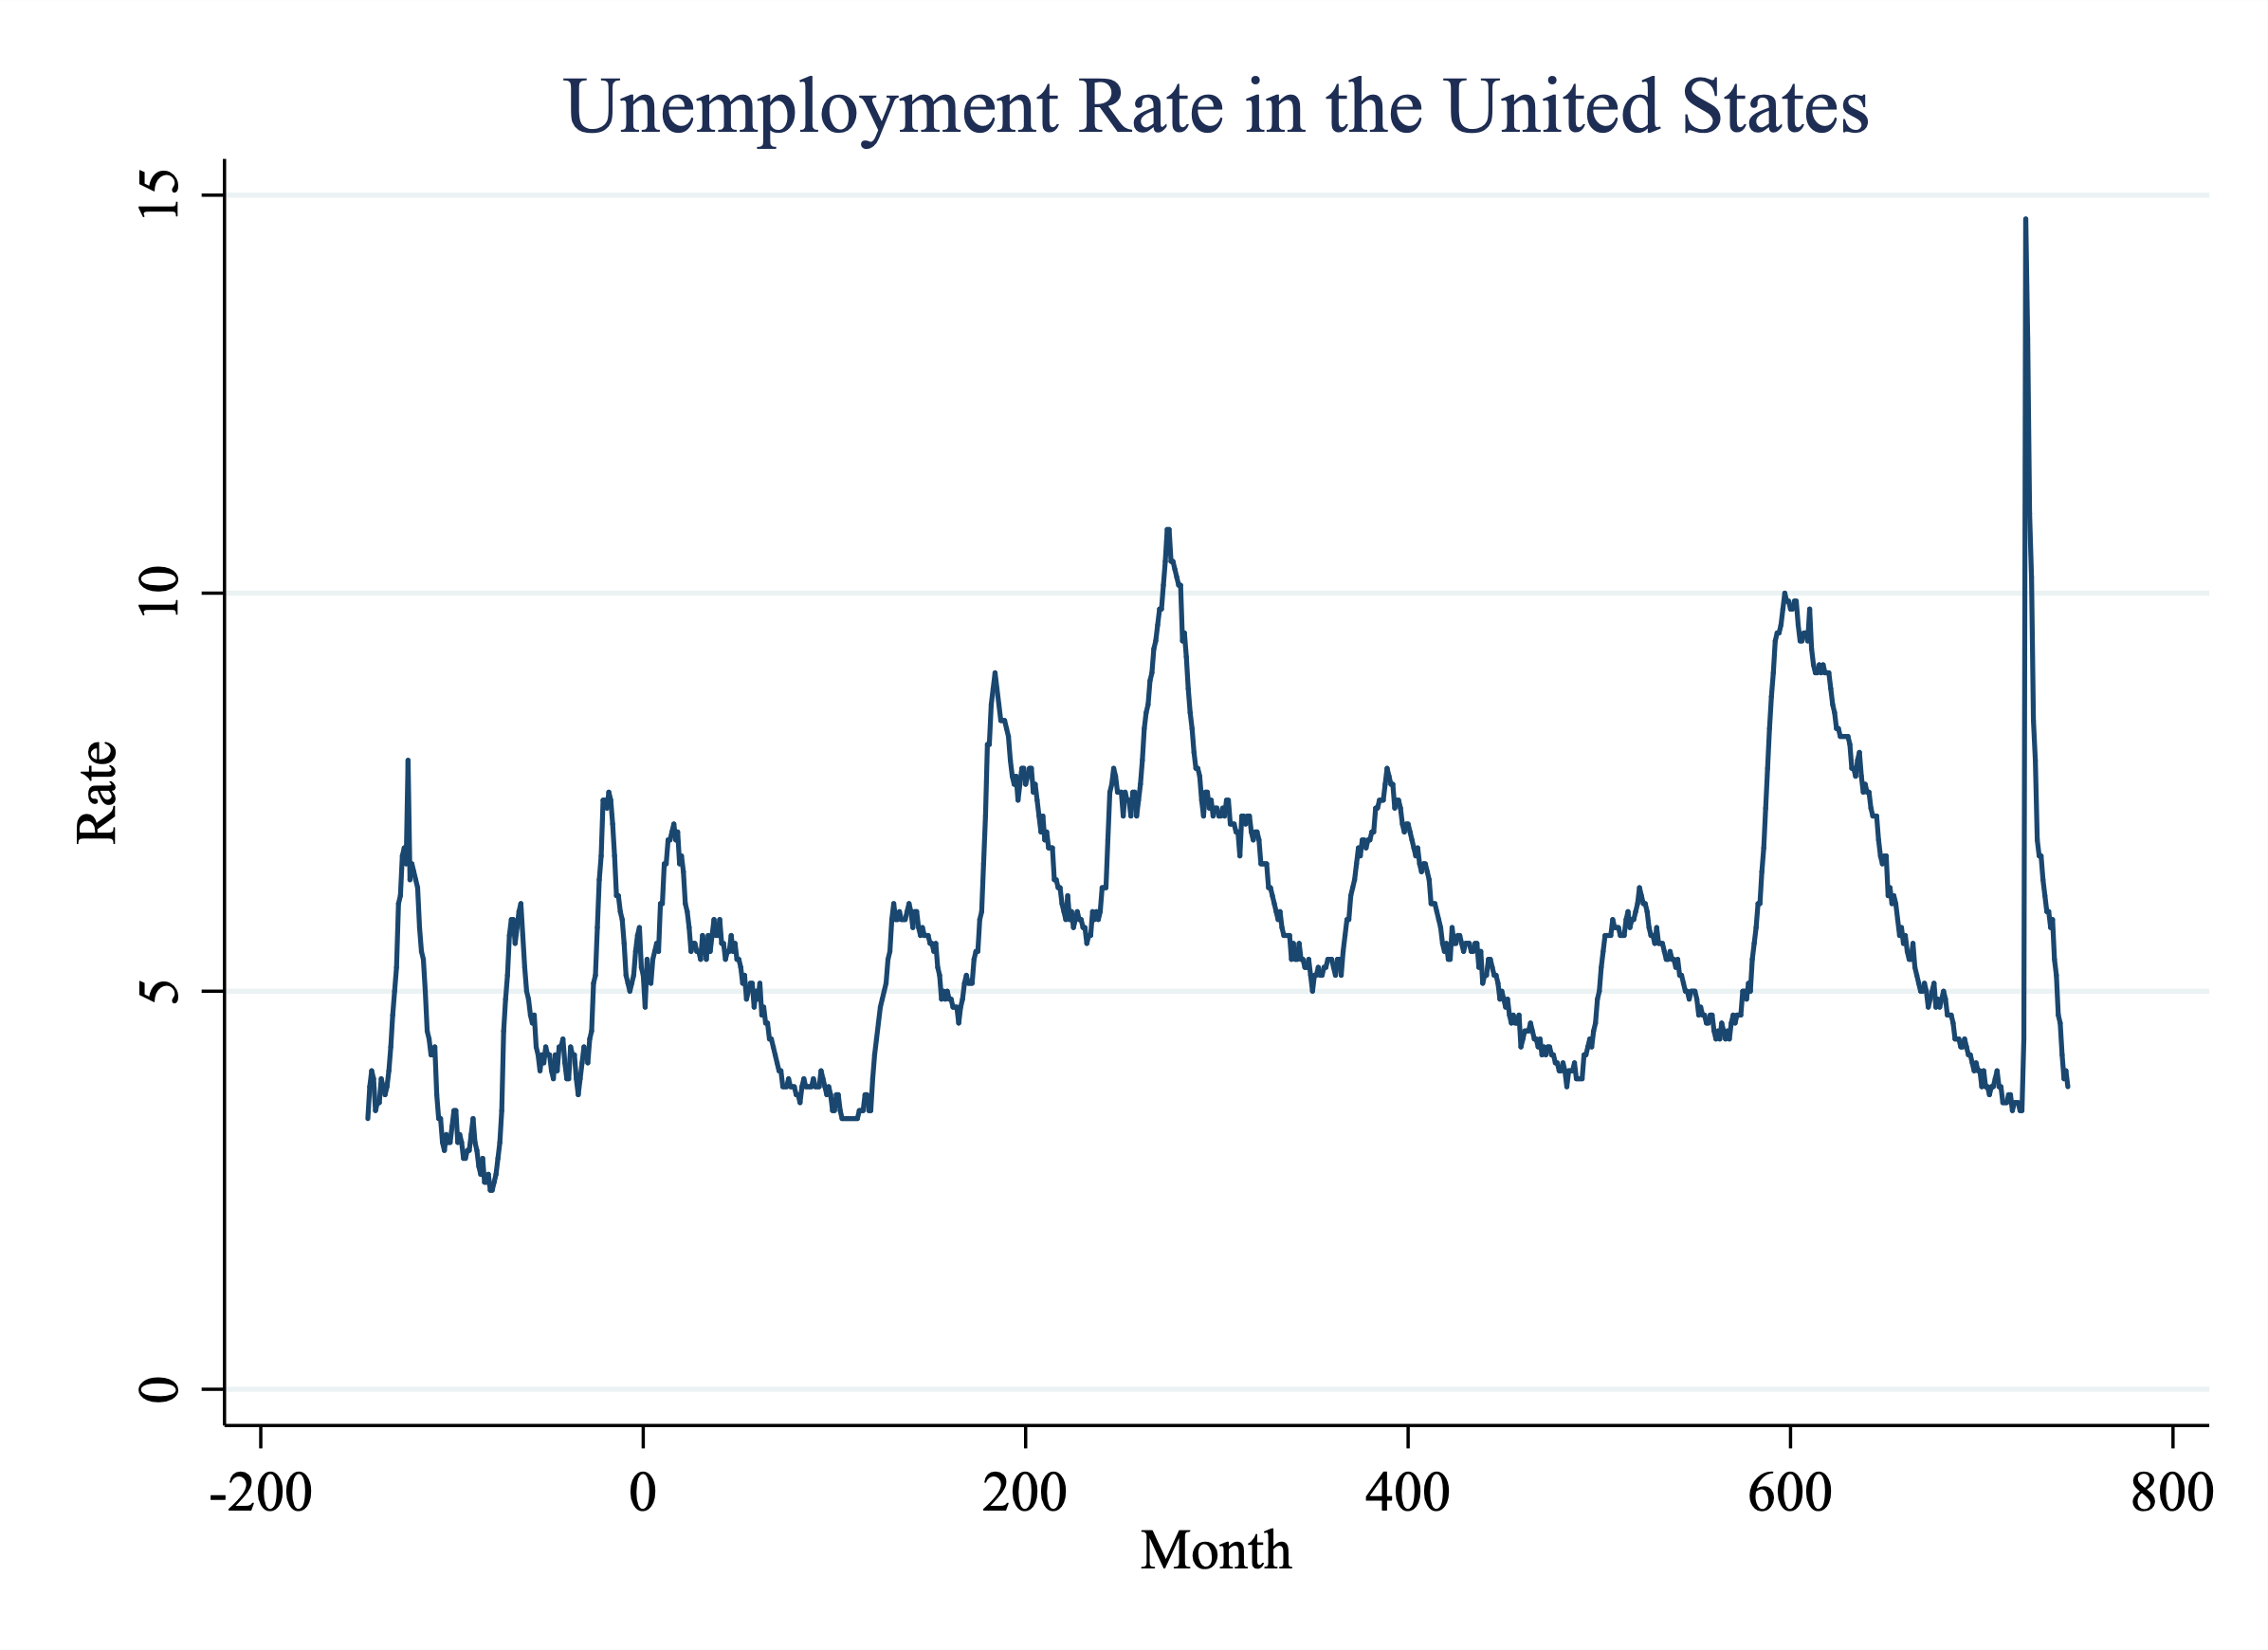
\includegraphics[scale=0.23]{Figures/Fig_6pt1.png}
\end{figure}
Unemployment is countercyclical, and has some long-run trends
\end{frame}

\begin{frame}
\frametitle[alignment=center]{Deviations from Trend in the US Unemployment Rate}
\begin{figure}
\centering
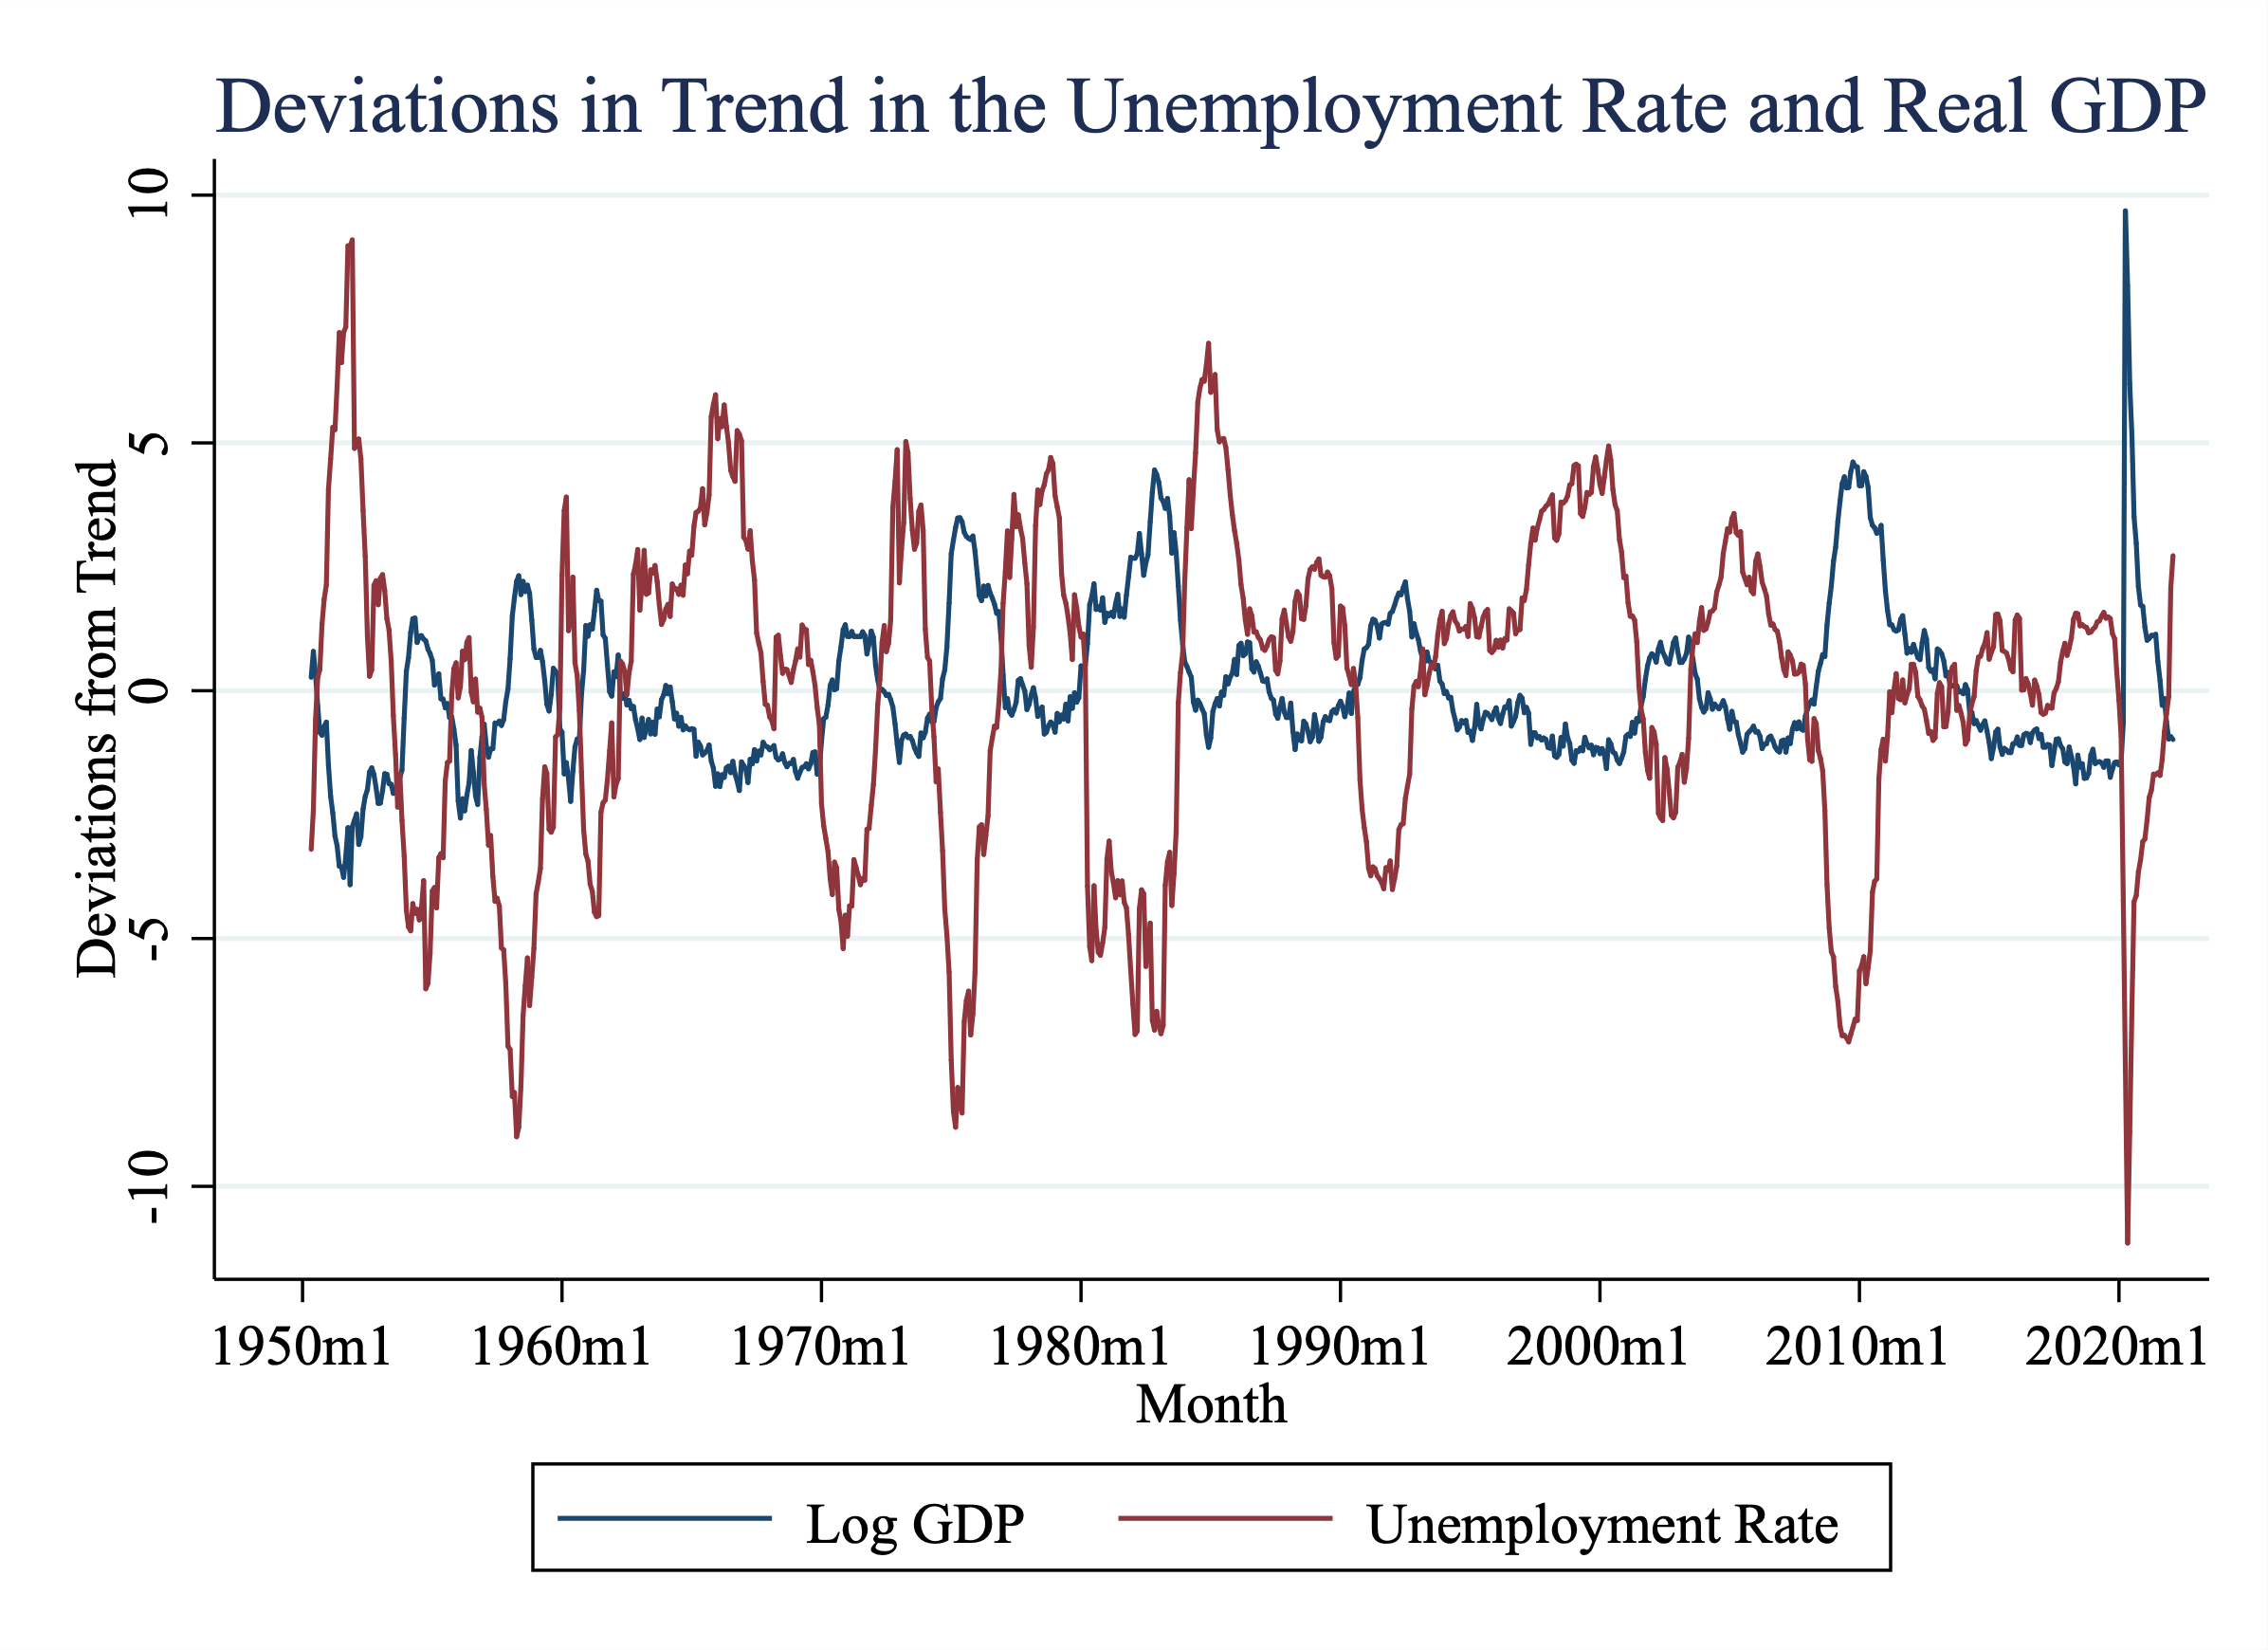
\includegraphics[scale=0.23]{Figures/Fig_6pt2.png}
\end{figure}
Unemployment is clearly countercyclical
\end{frame}

\begin{frame}
\frametitle[alignment=center]{Labor Force Participation Rate}
\begin{figure}
\centering
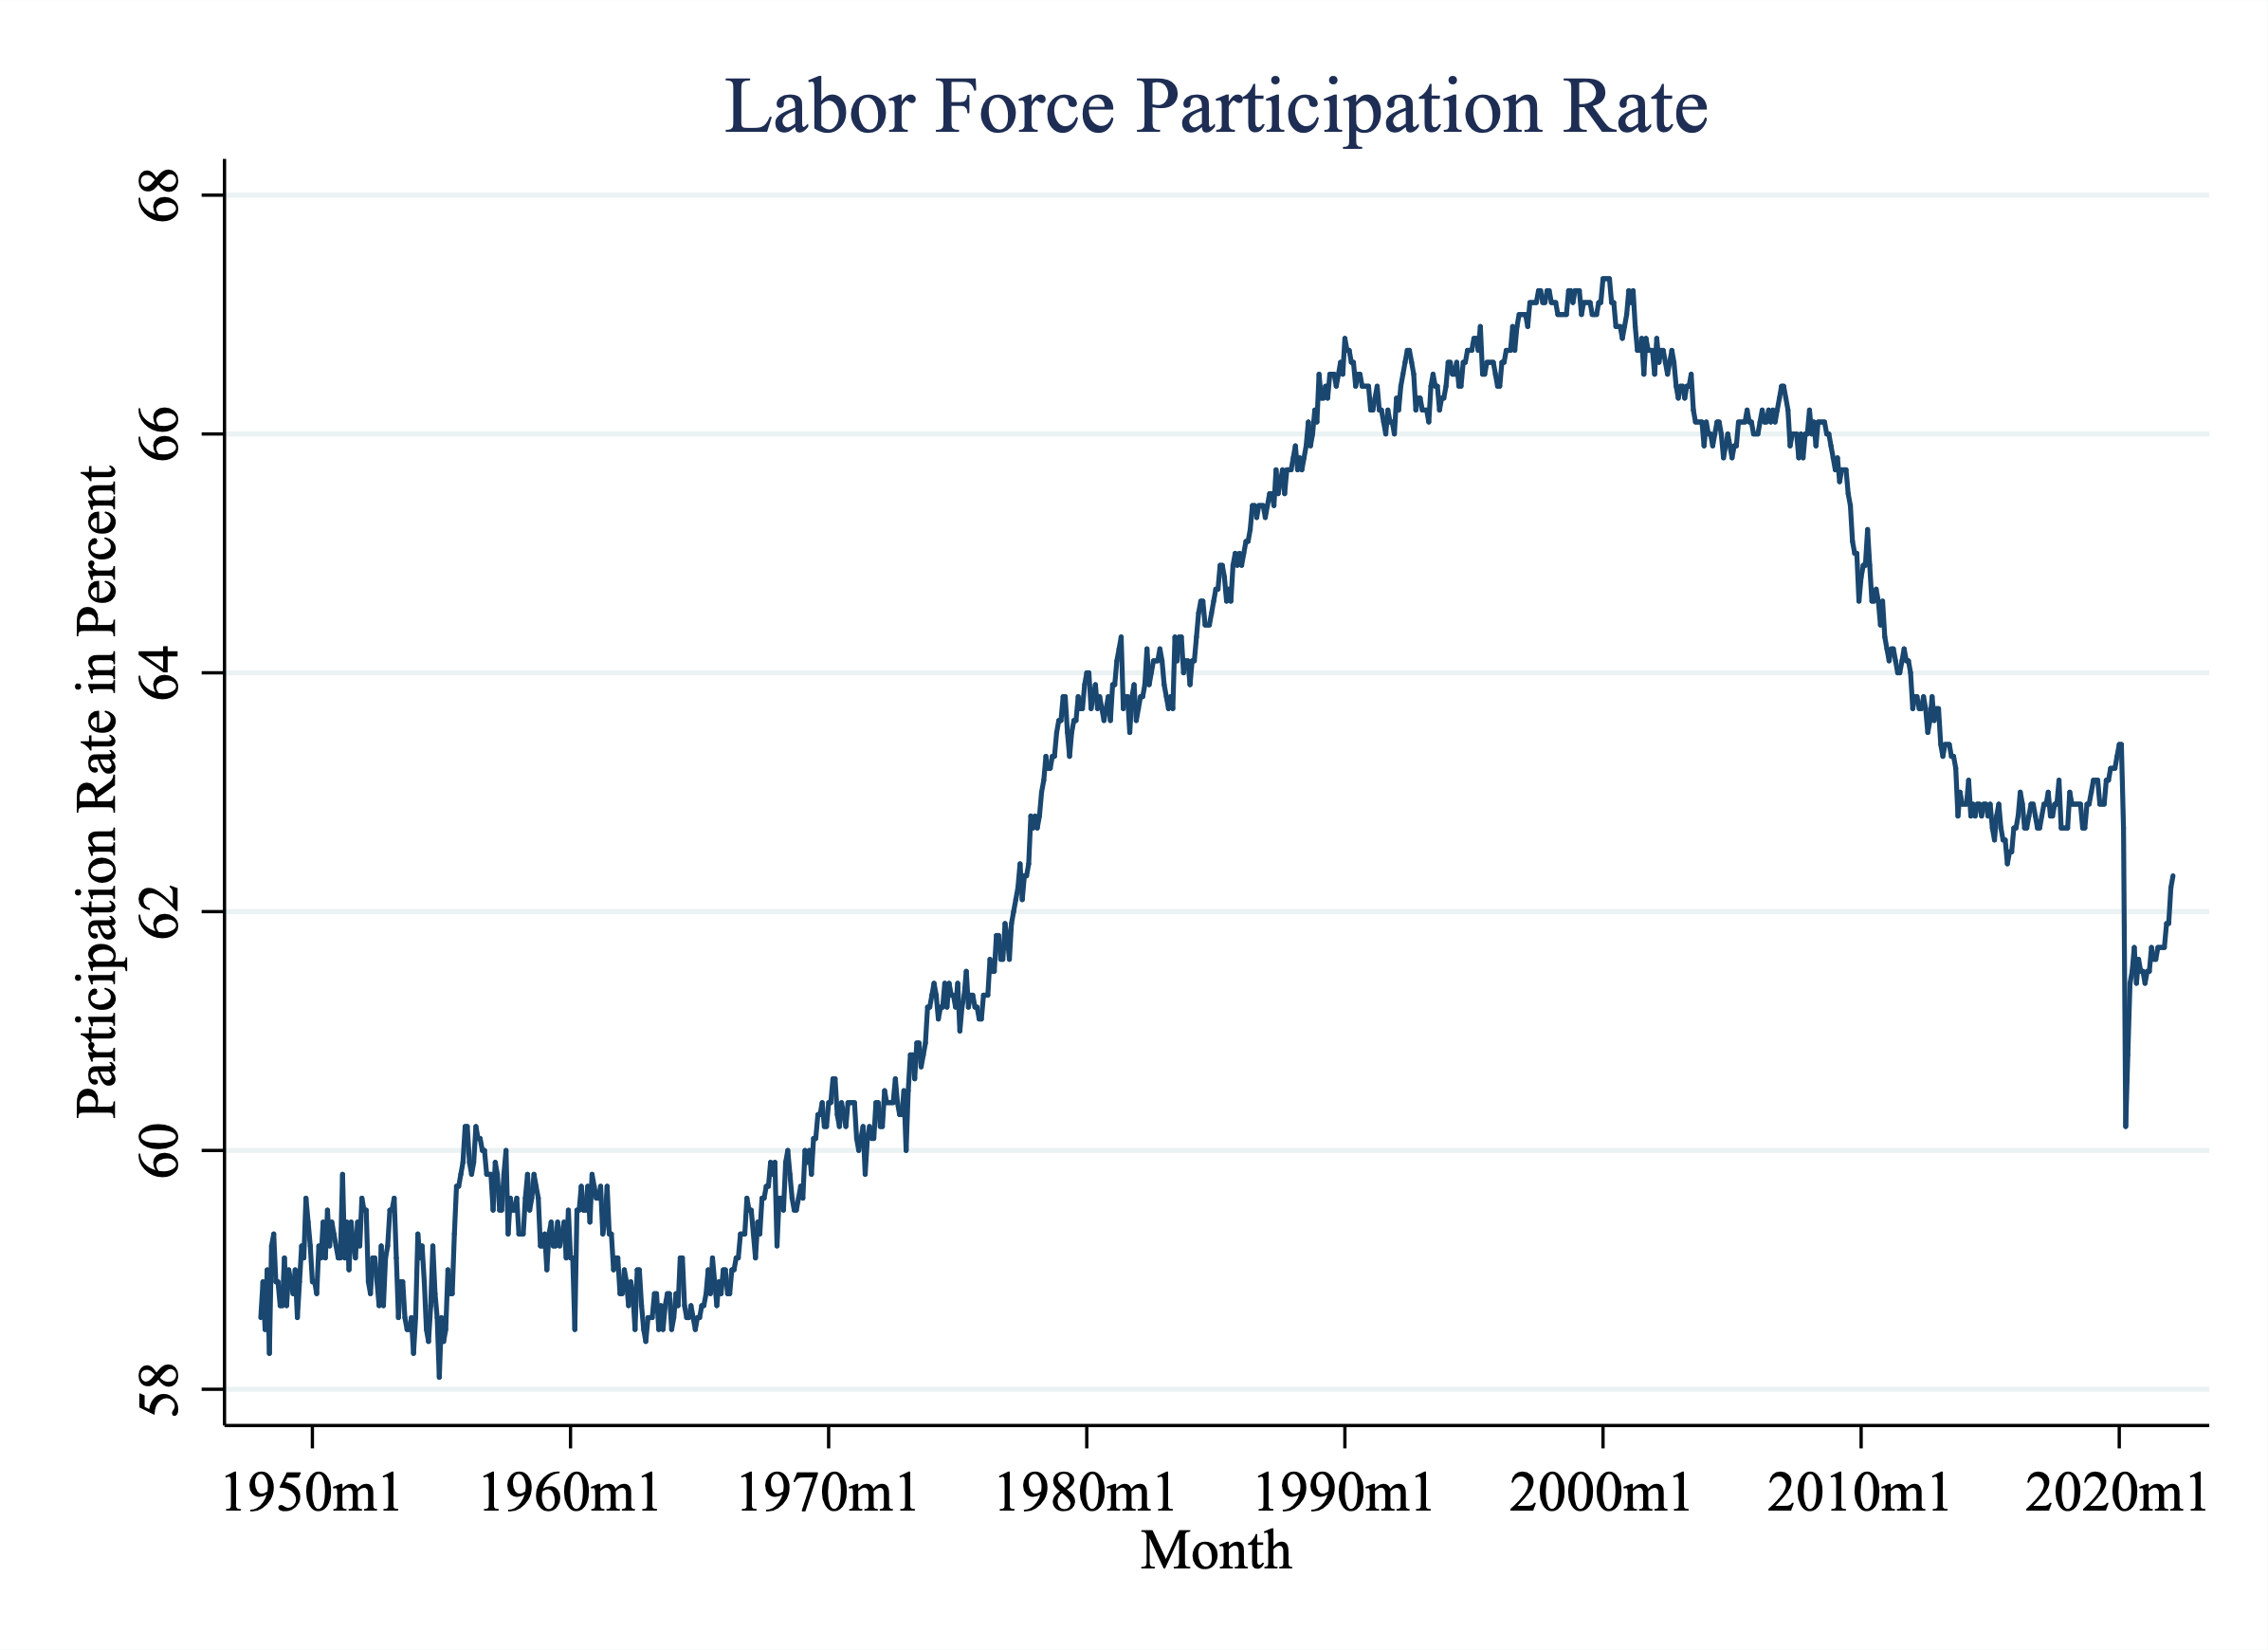
\includegraphics[scale=0.23]{Figures/Fig_6pt3.png}
\end{figure}
Stark long-run changes in the Labor Force Participation Rate
\end{frame}

\begin{frame}
\frametitle[alignment=center]{Labor Force Participation Rates of Men and Women}
\begin{figure}
\centering
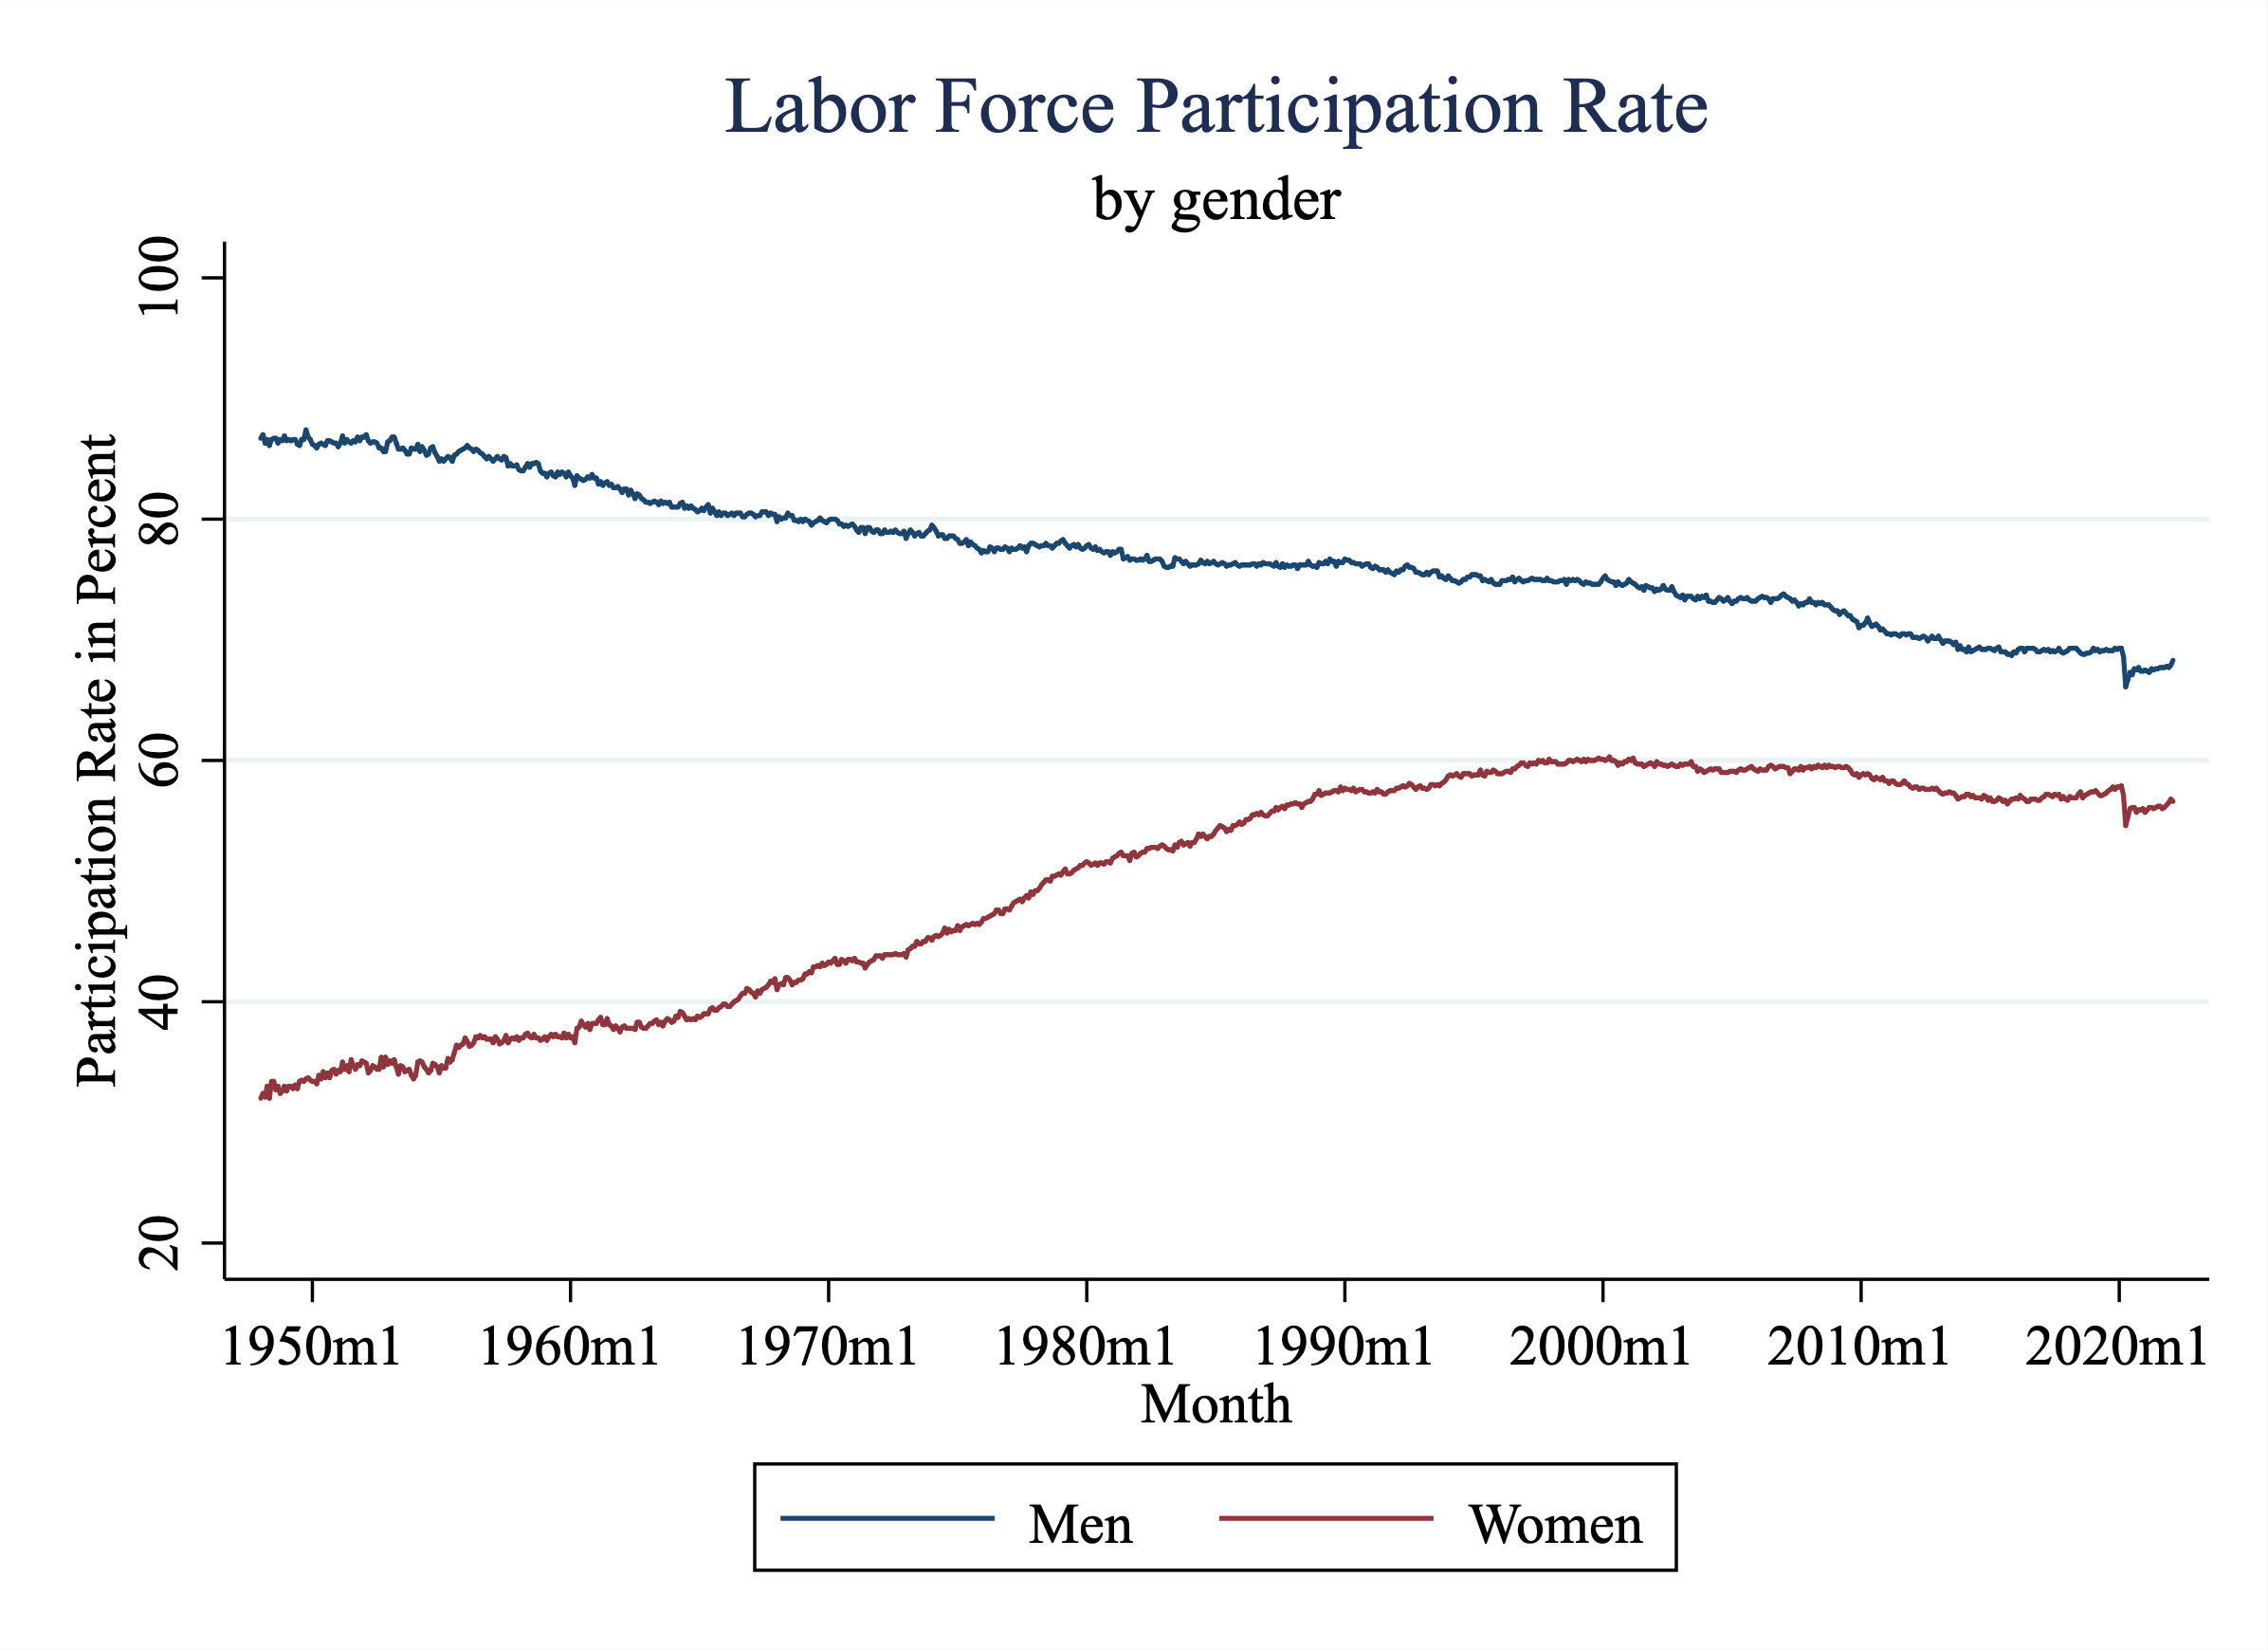
\includegraphics[scale=0.23]{Figures/Fig_6pt4.png}
\end{figure}
Highly heterogeneous long-run trends by gender!
\end{frame}

\begin{frame}
\frametitle[alignment=center]{Percentage Devaitions from Trend in the Labor Force Participation Rate and Real GDP}
\begin{figure}
\centering
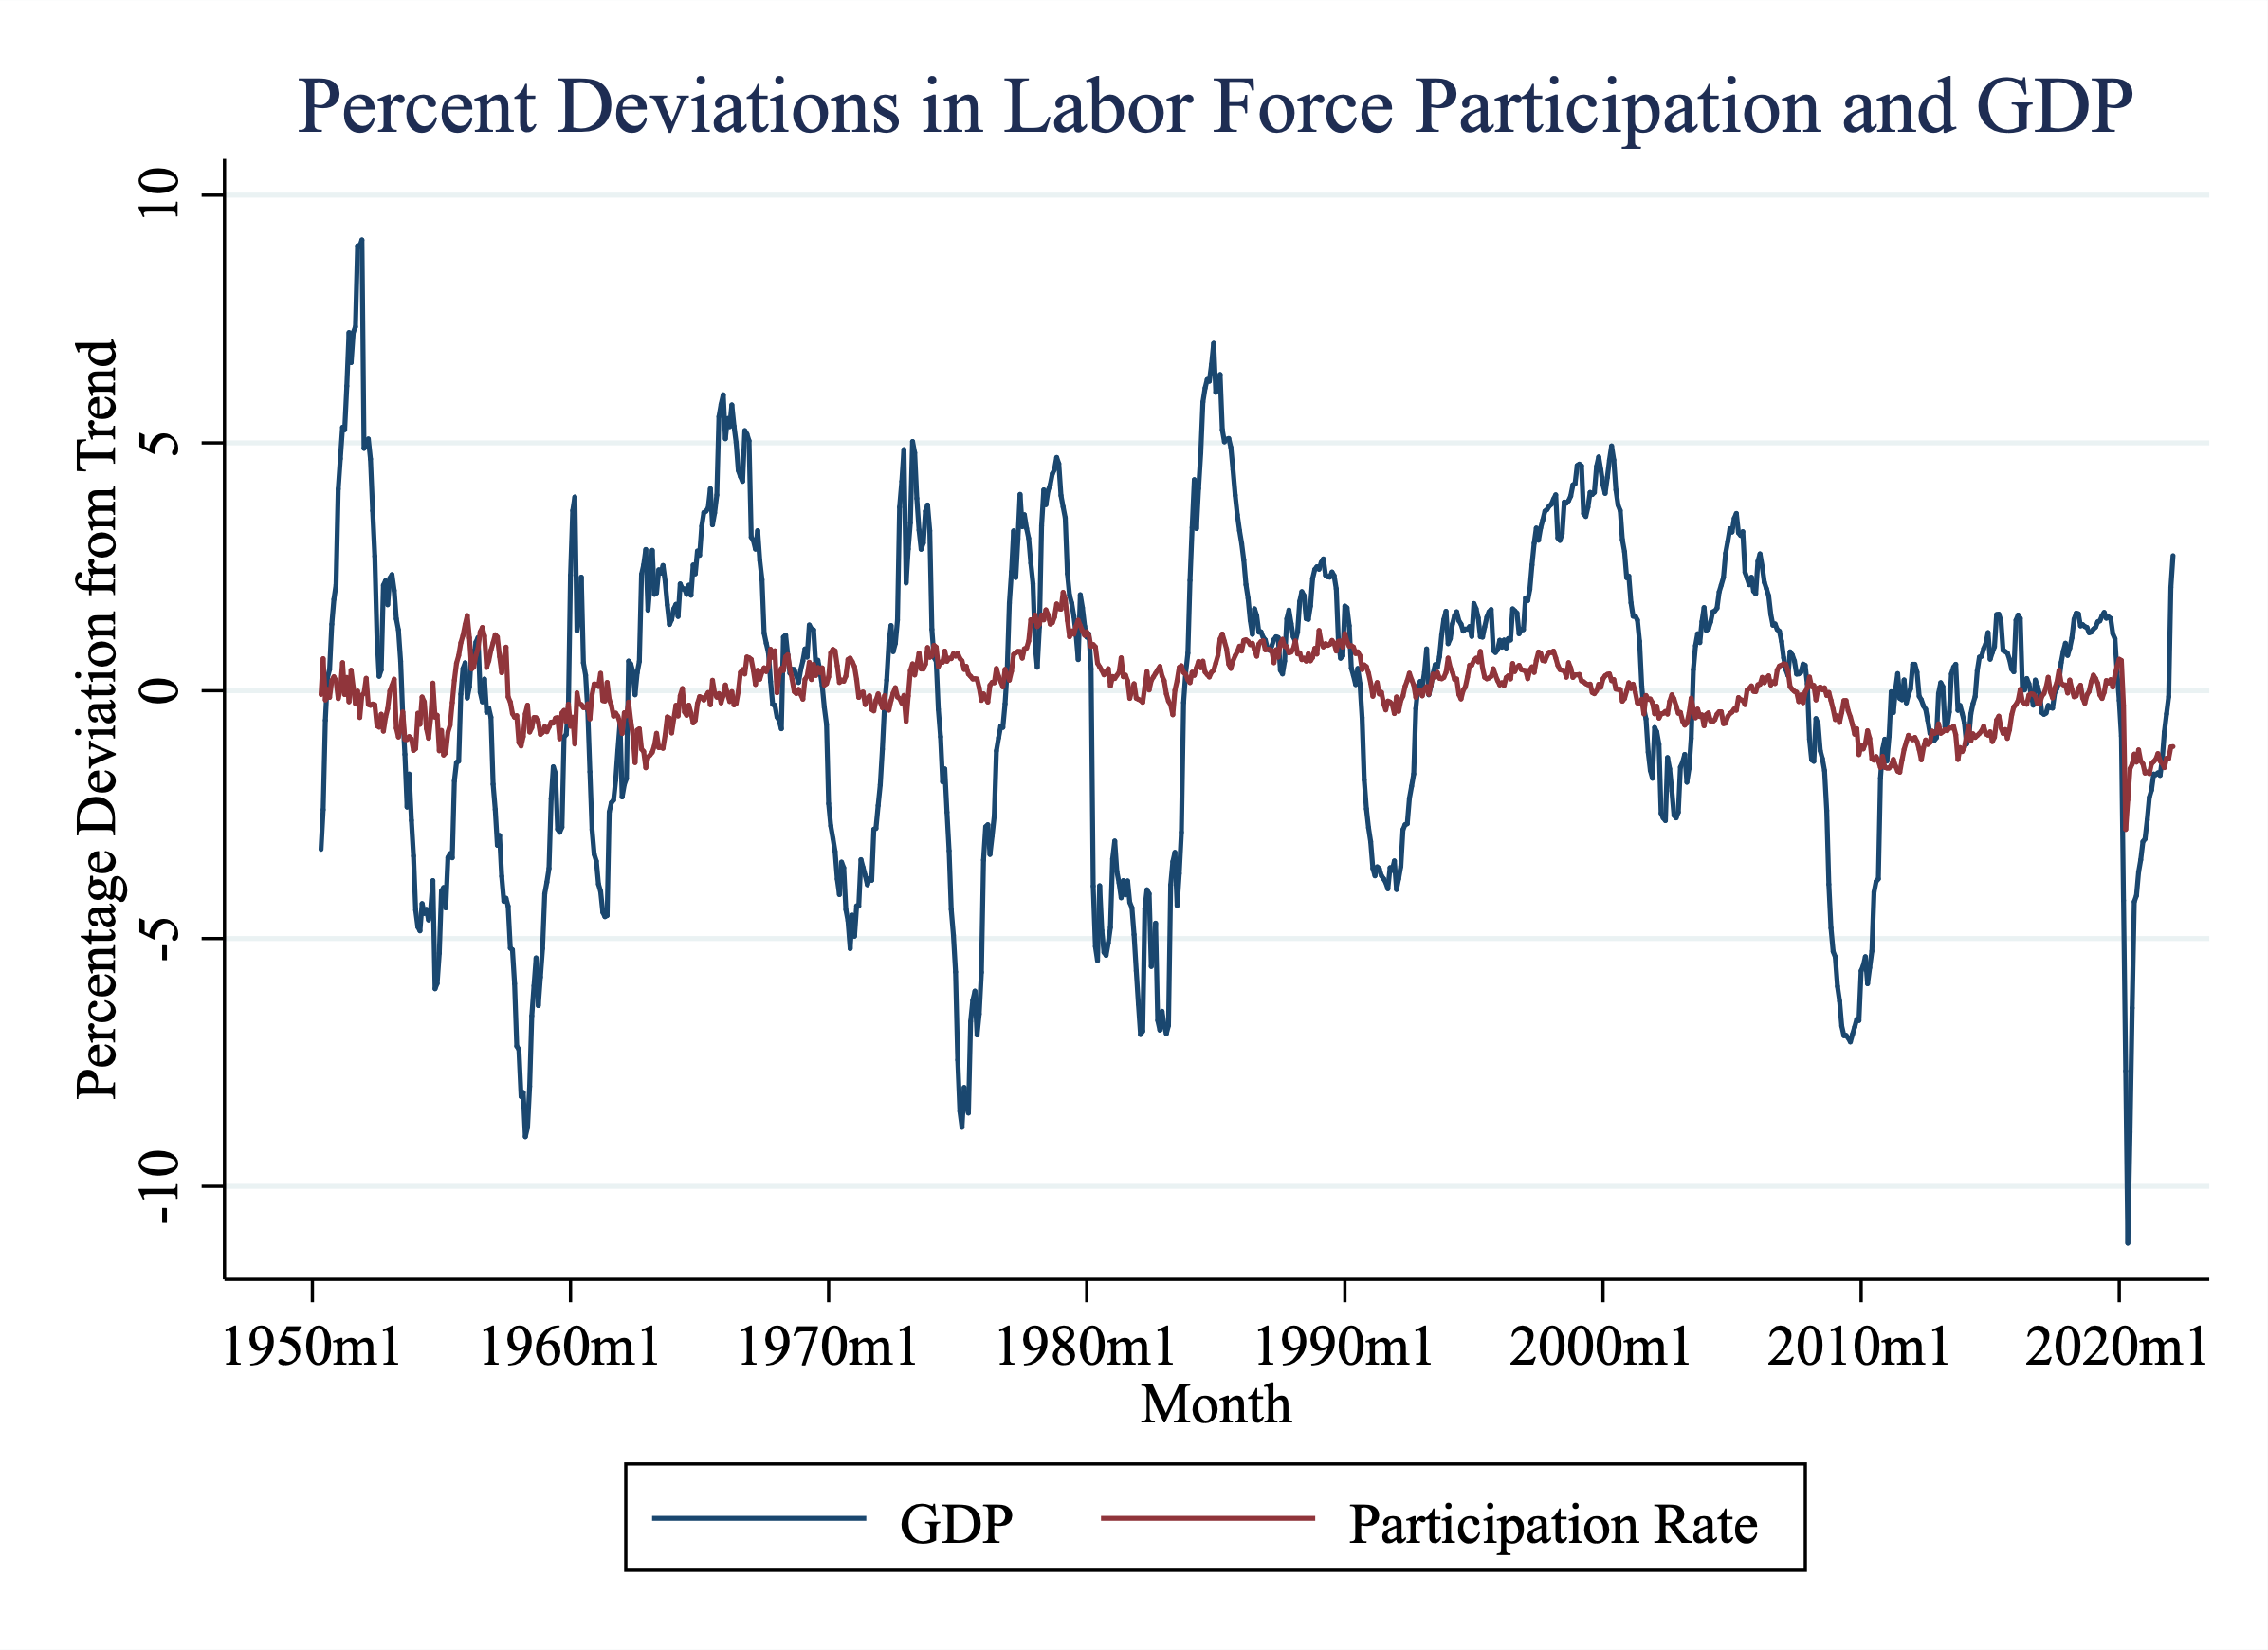
\includegraphics[scale=0.23]{Figures/Fig_6pt5.png}
\end{figure}
\end{frame}

\begin{frame}
\frametitle[alignment=center]{Labor Force Participation Rate and Employment/Population Ratio}
\begin{figure}
\centering
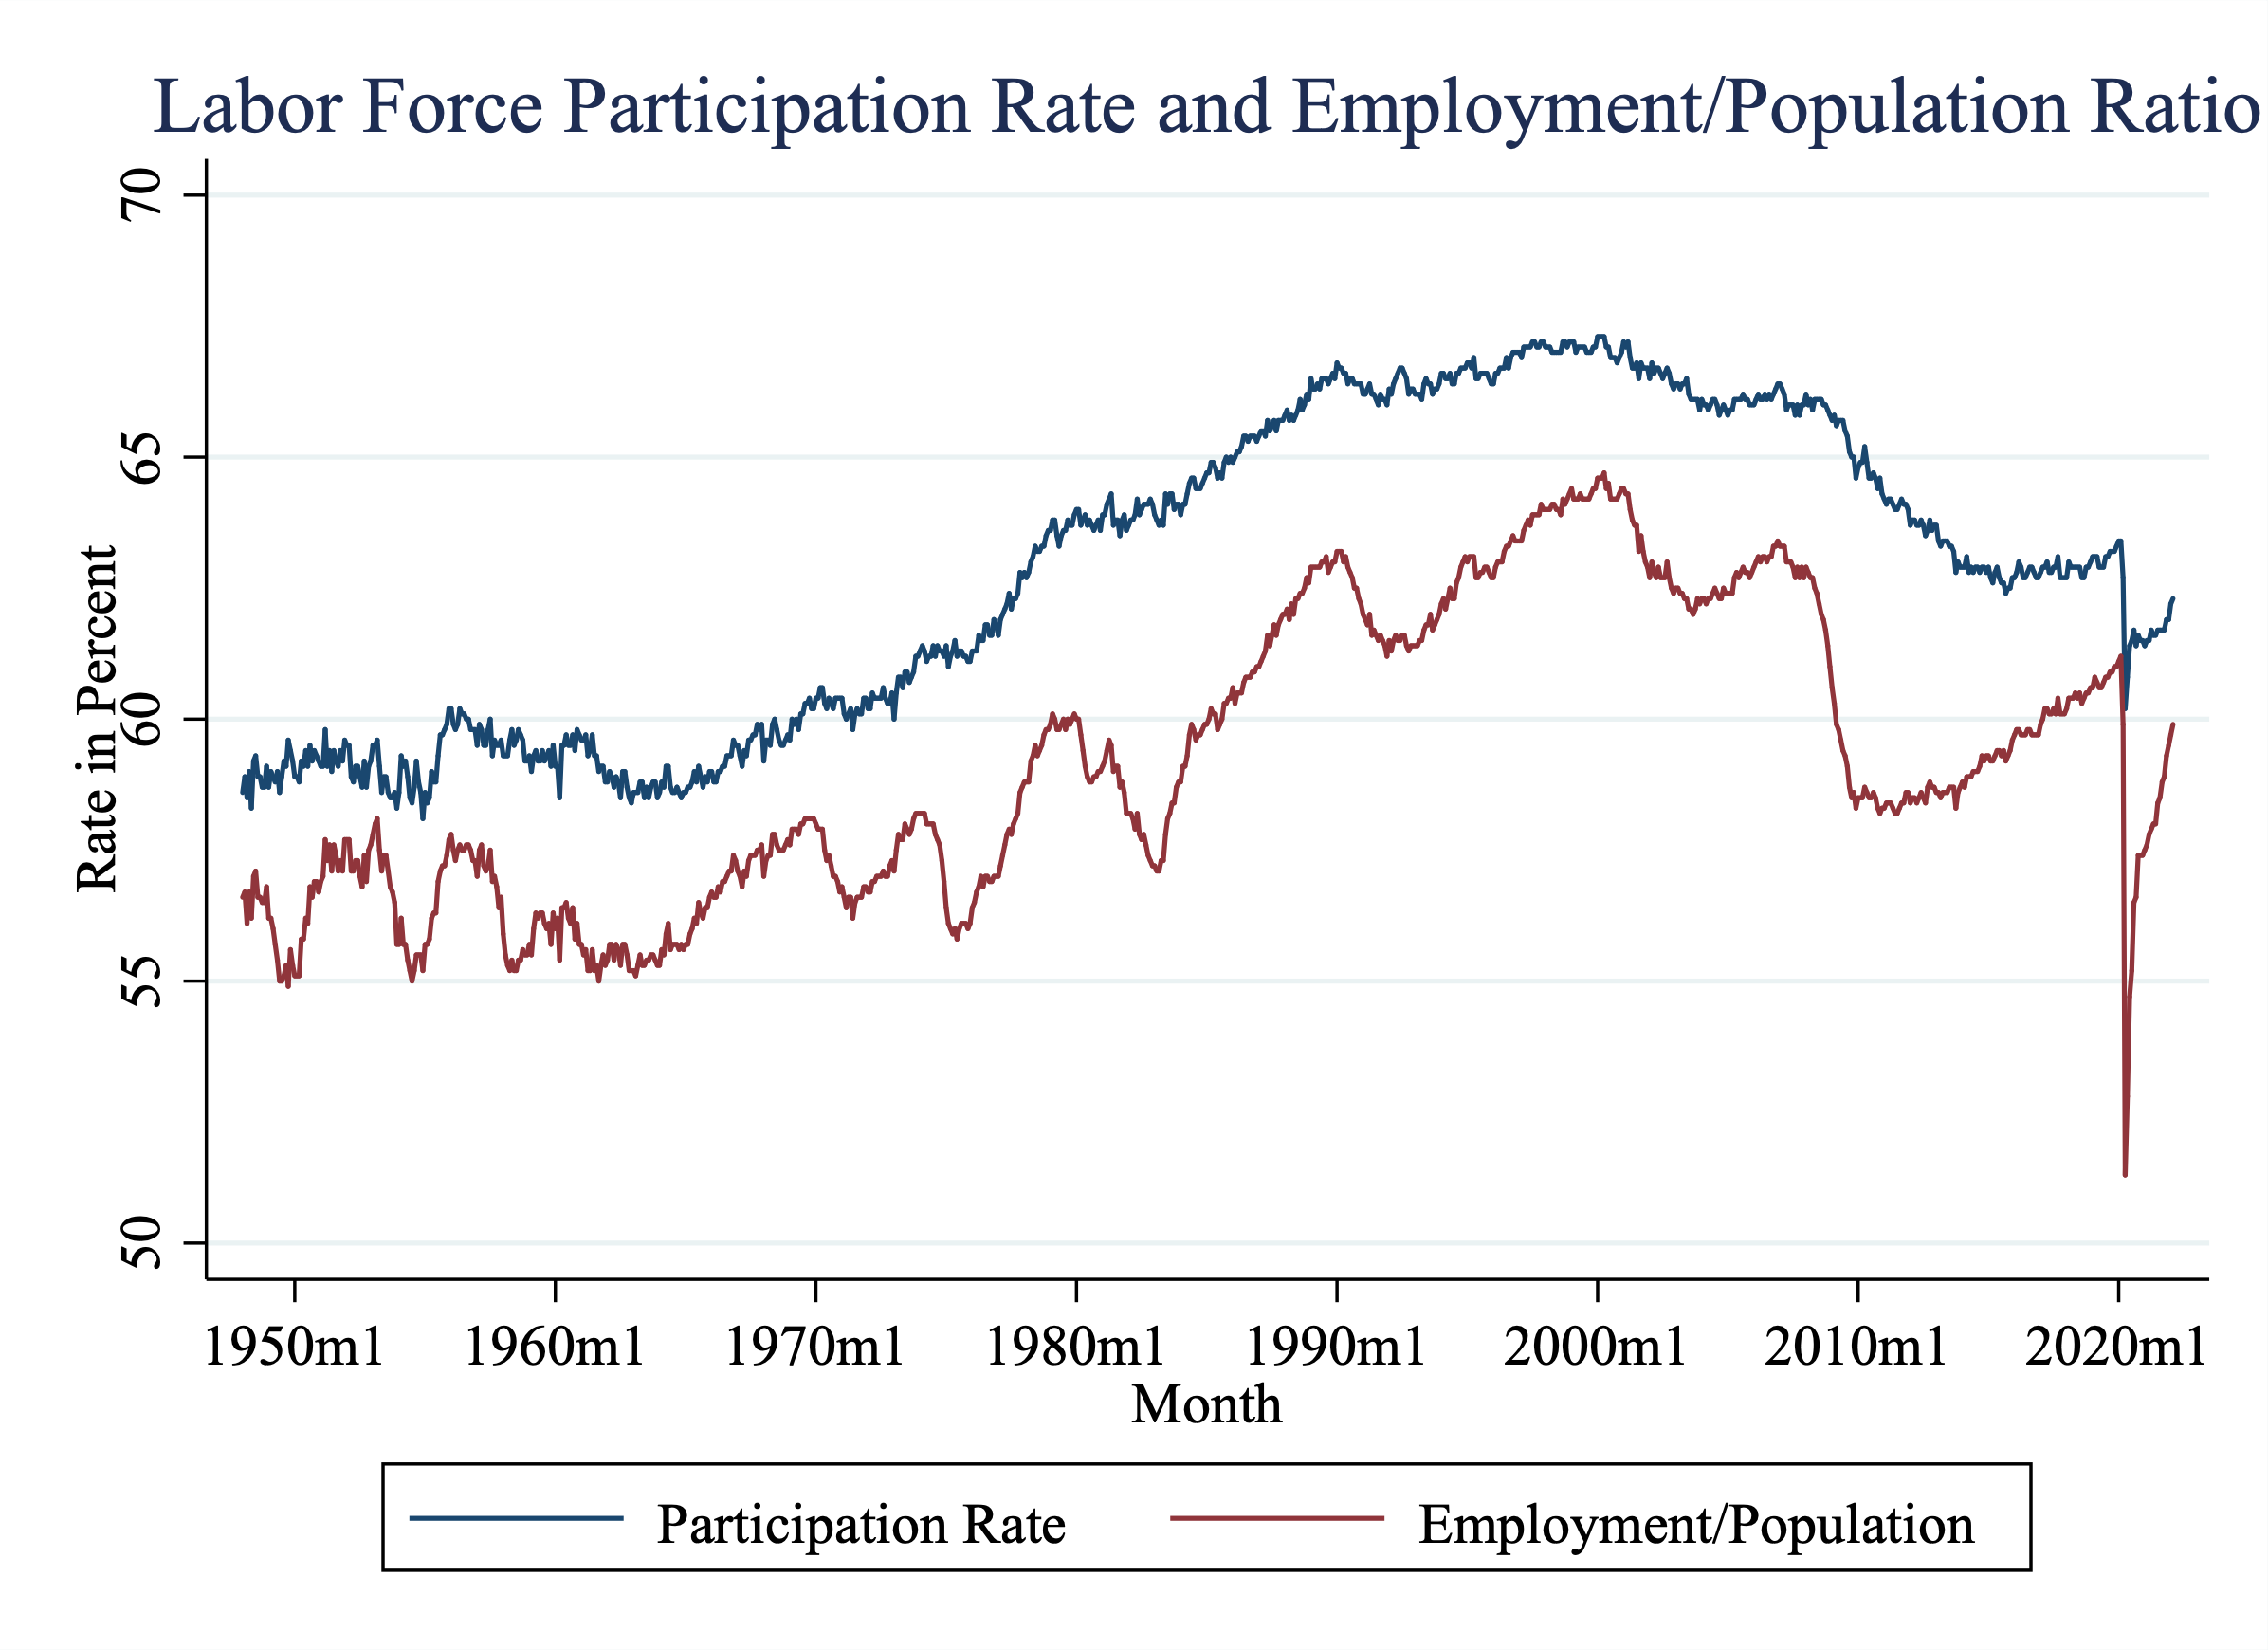
\includegraphics[scale=0.23]{Figures/Fig_6pt6.png}
\end{figure}
Participation rate is procyclical, but much less volatile than real GDP (unlike U)
\end{frame}

\begin{frame}
\frametitle[alignment=center]{Vacancy Rate and the Beveridge Curve}
\begin{itemize}
\item We think of workers as the only ``unemployed" people, but the problem is symmetric! (like dating!)
\bigskip
\item Vacancies are ``unemployed" firms:  firms advertise job vacancies ($A$) they wish to fill
\bigskip
\item Unfilled jobs are costly to firms (otherwise, why hire?)
\bigskip
\item Define the vacancy rate as: 
$$\text{vacancy rate}=\frac{A}{A+\mathcal{Q}-U}$$
\item Num vacancies / number of vacancies+employed, just like unemployment
\end{itemize}
\end{frame}

\begin{frame}
\frametitle[alignment=center]{Vacancy Rate and the Unemployment Rate}
\begin{figure}
\centering
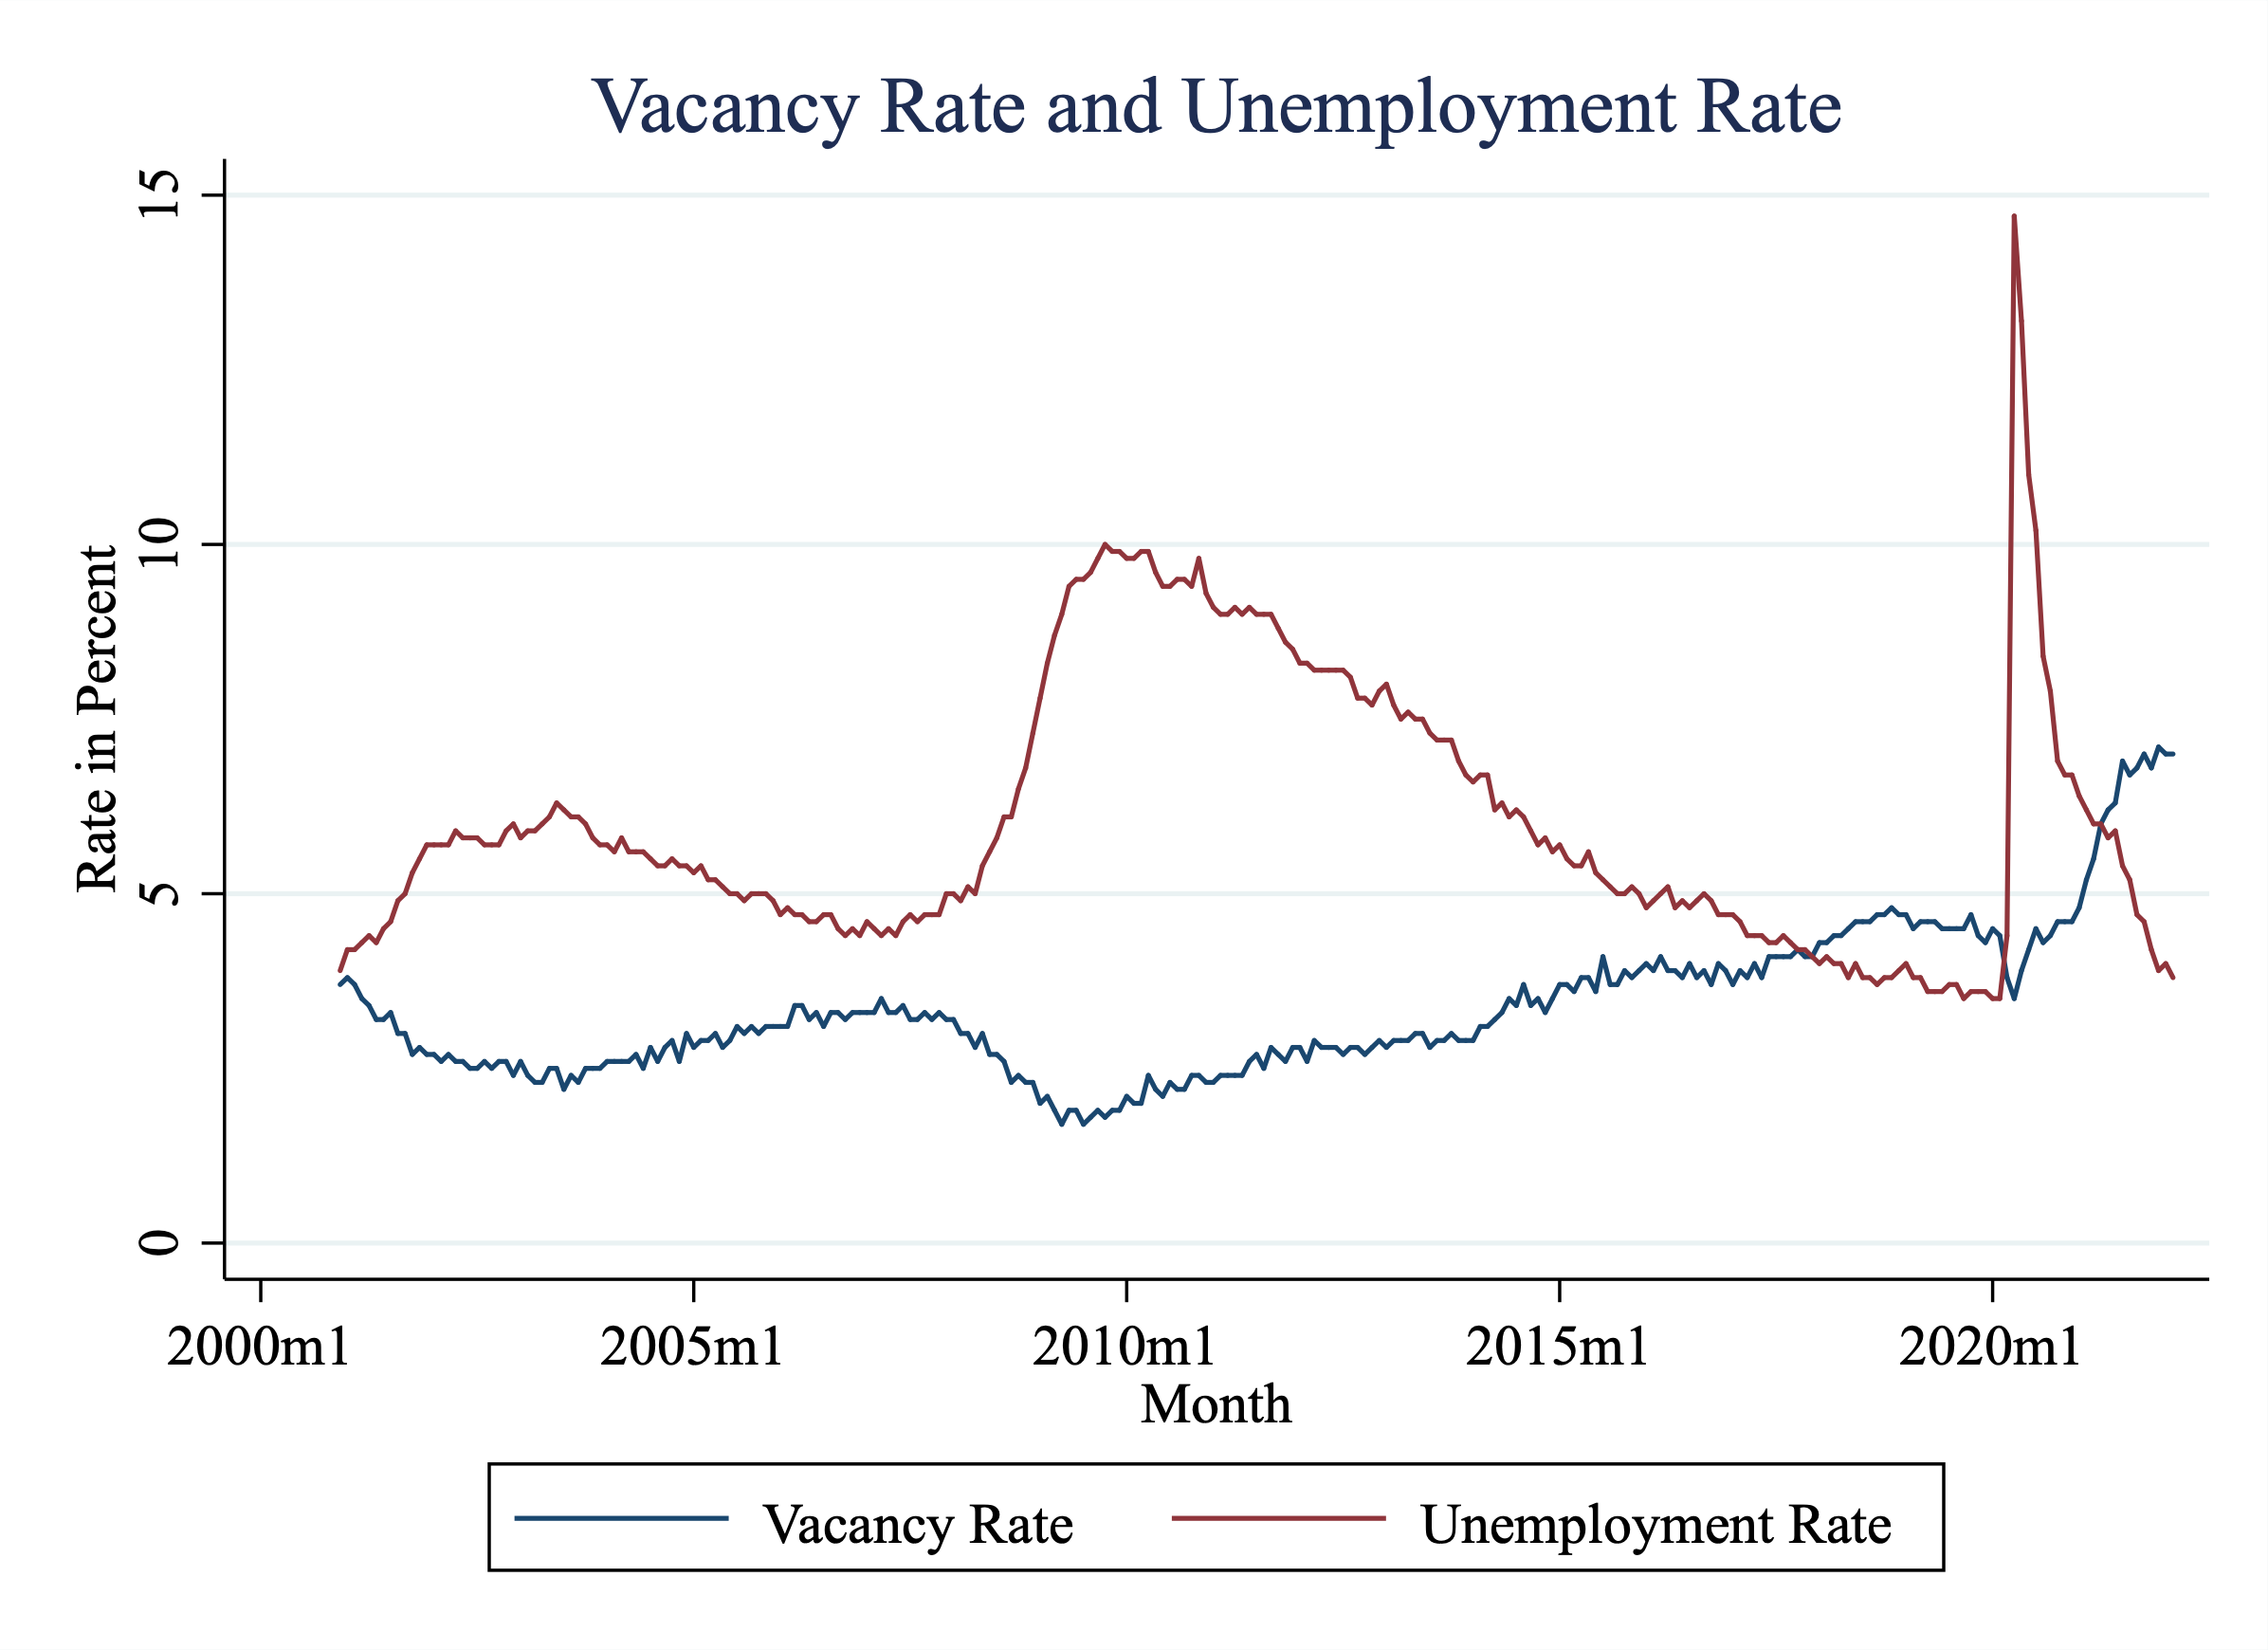
\includegraphics[scale=0.25]{Figures/Fig_6pt7.png}
\end{figure}
\end{frame}

\begin{frame}
\frametitle[alignment=center]{Vacancy Rate and the Unemployment Rate}
\begin{figure}
\centering
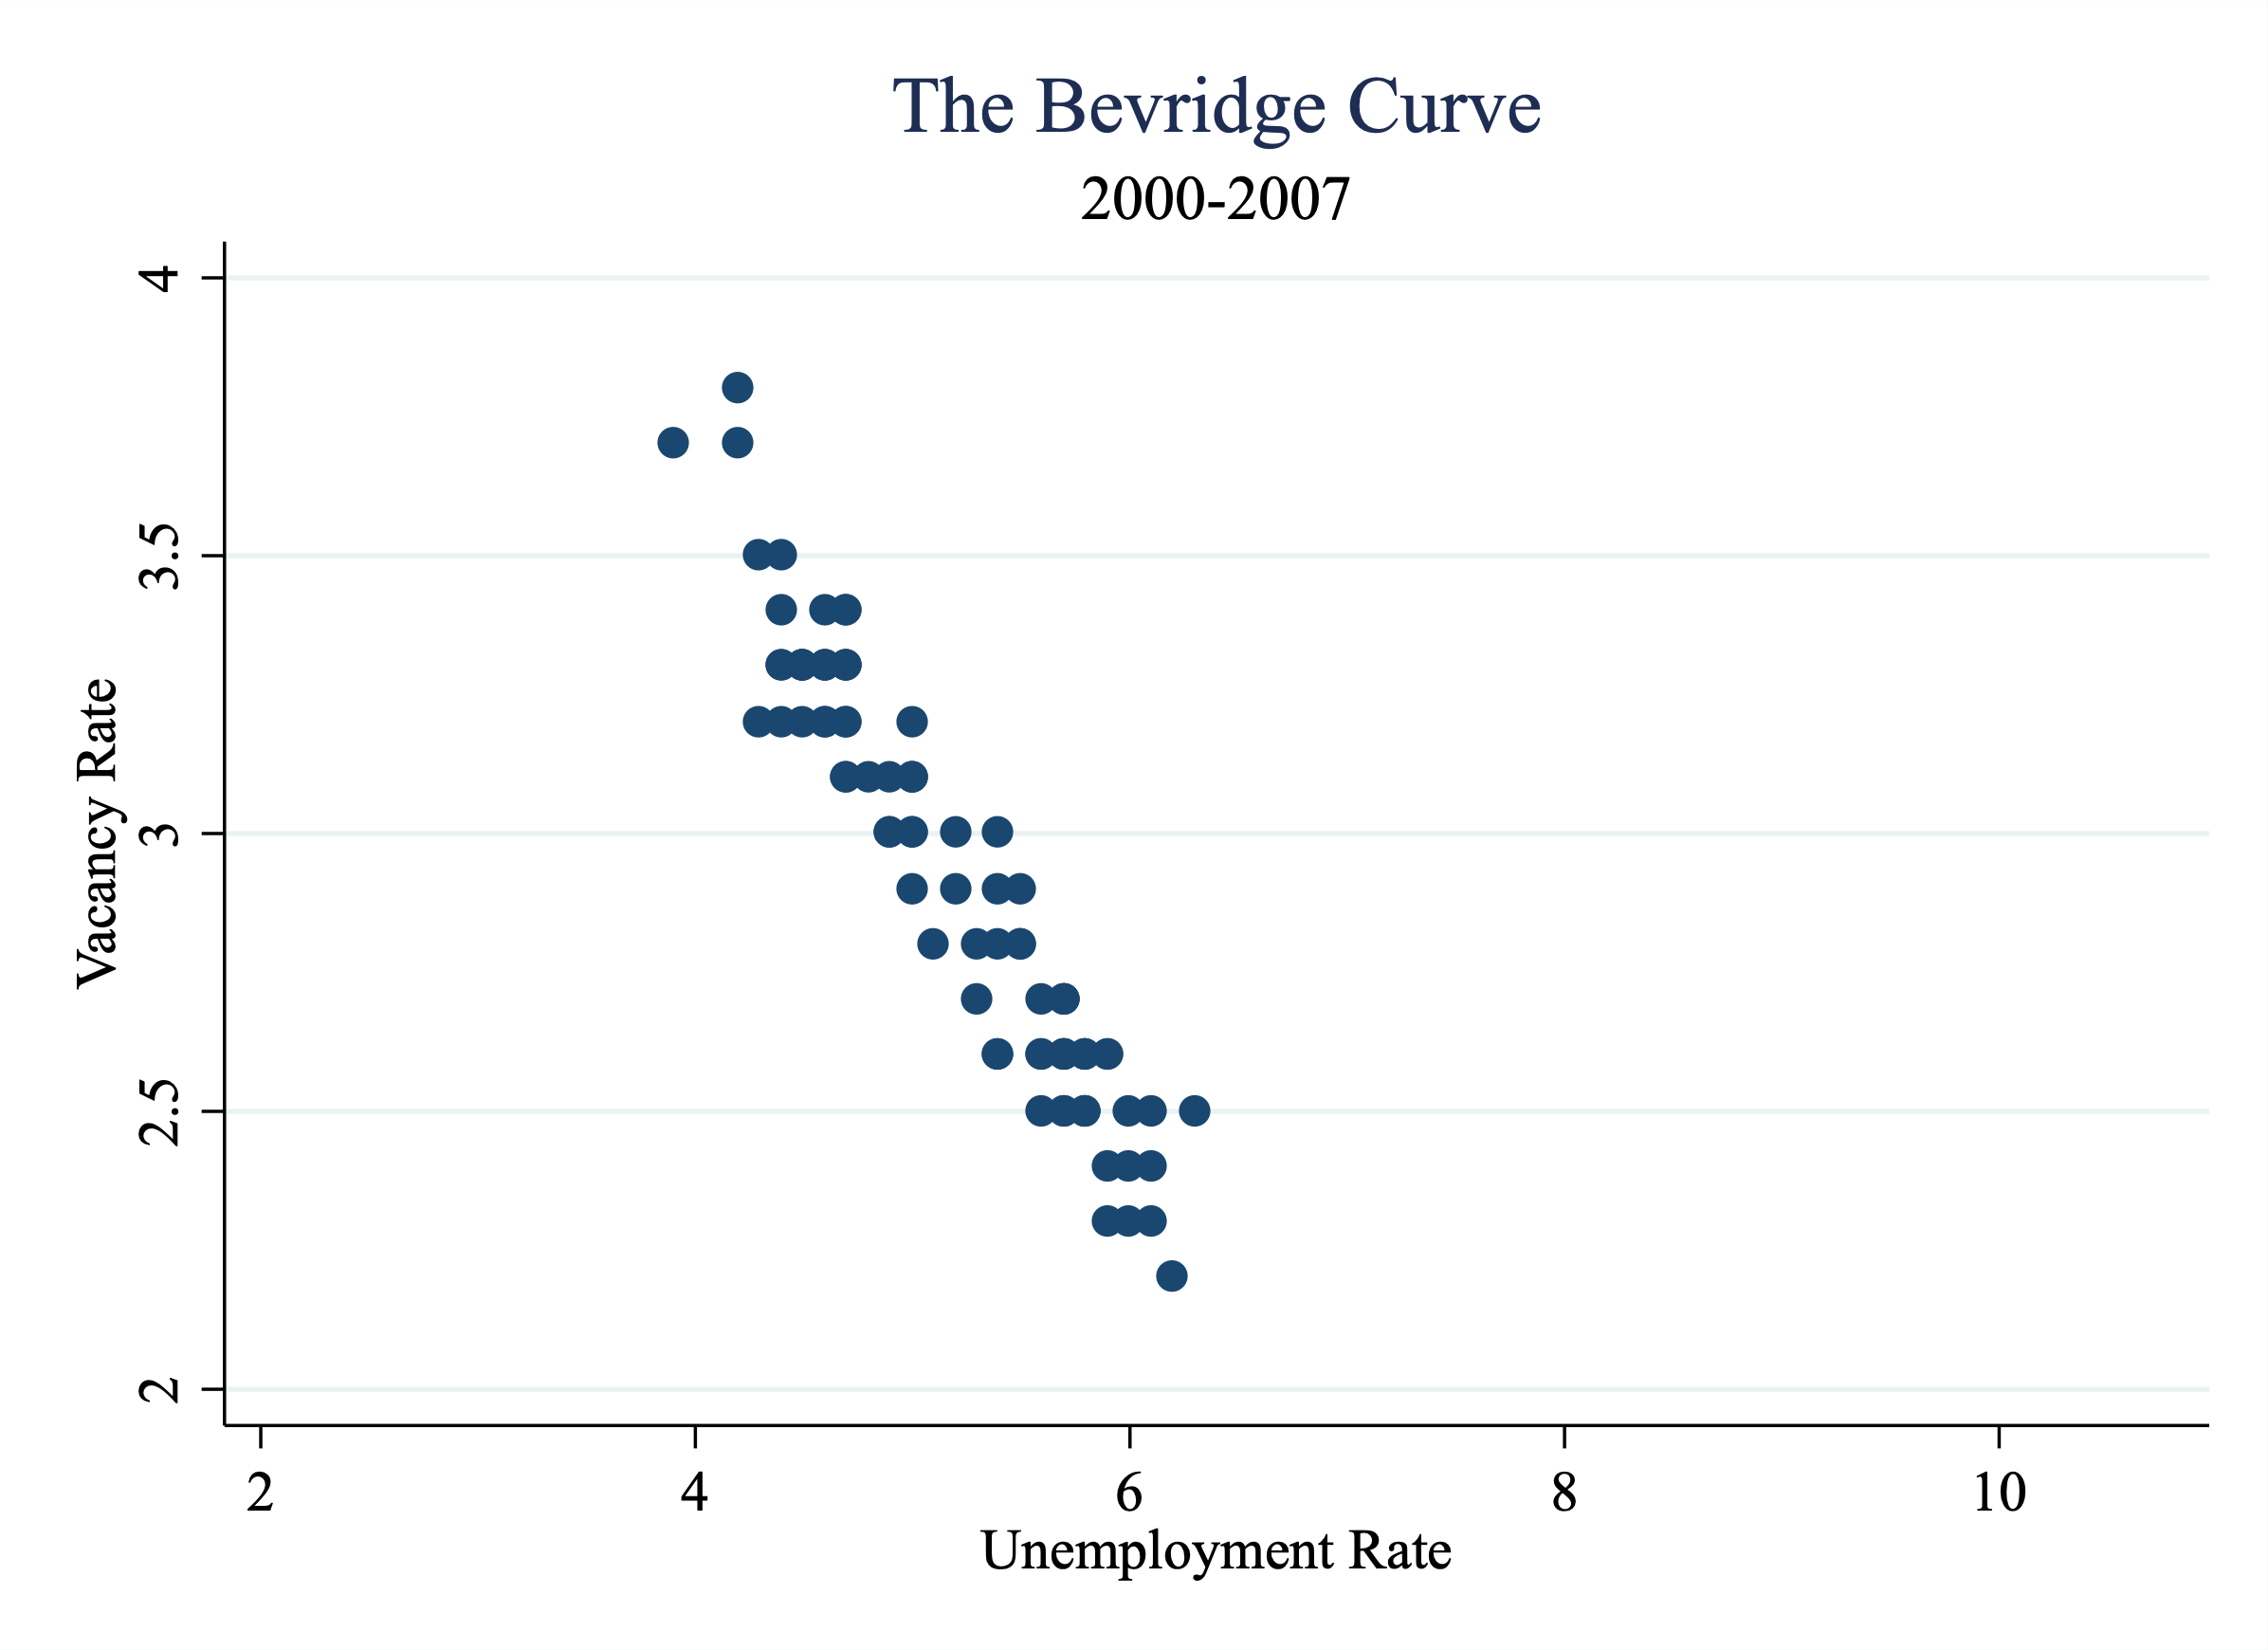
\includegraphics[scale=0.23]{Figures/Beverige_Initial.png}
\end{figure}
Pretty important!  Tight empirical relationship we can really build a science on right?
\end{frame}

\begin{frame}
\frametitle[alignment=center]{Vacancy Rate and the Unemployment Rate}
\begin{figure}
\centering
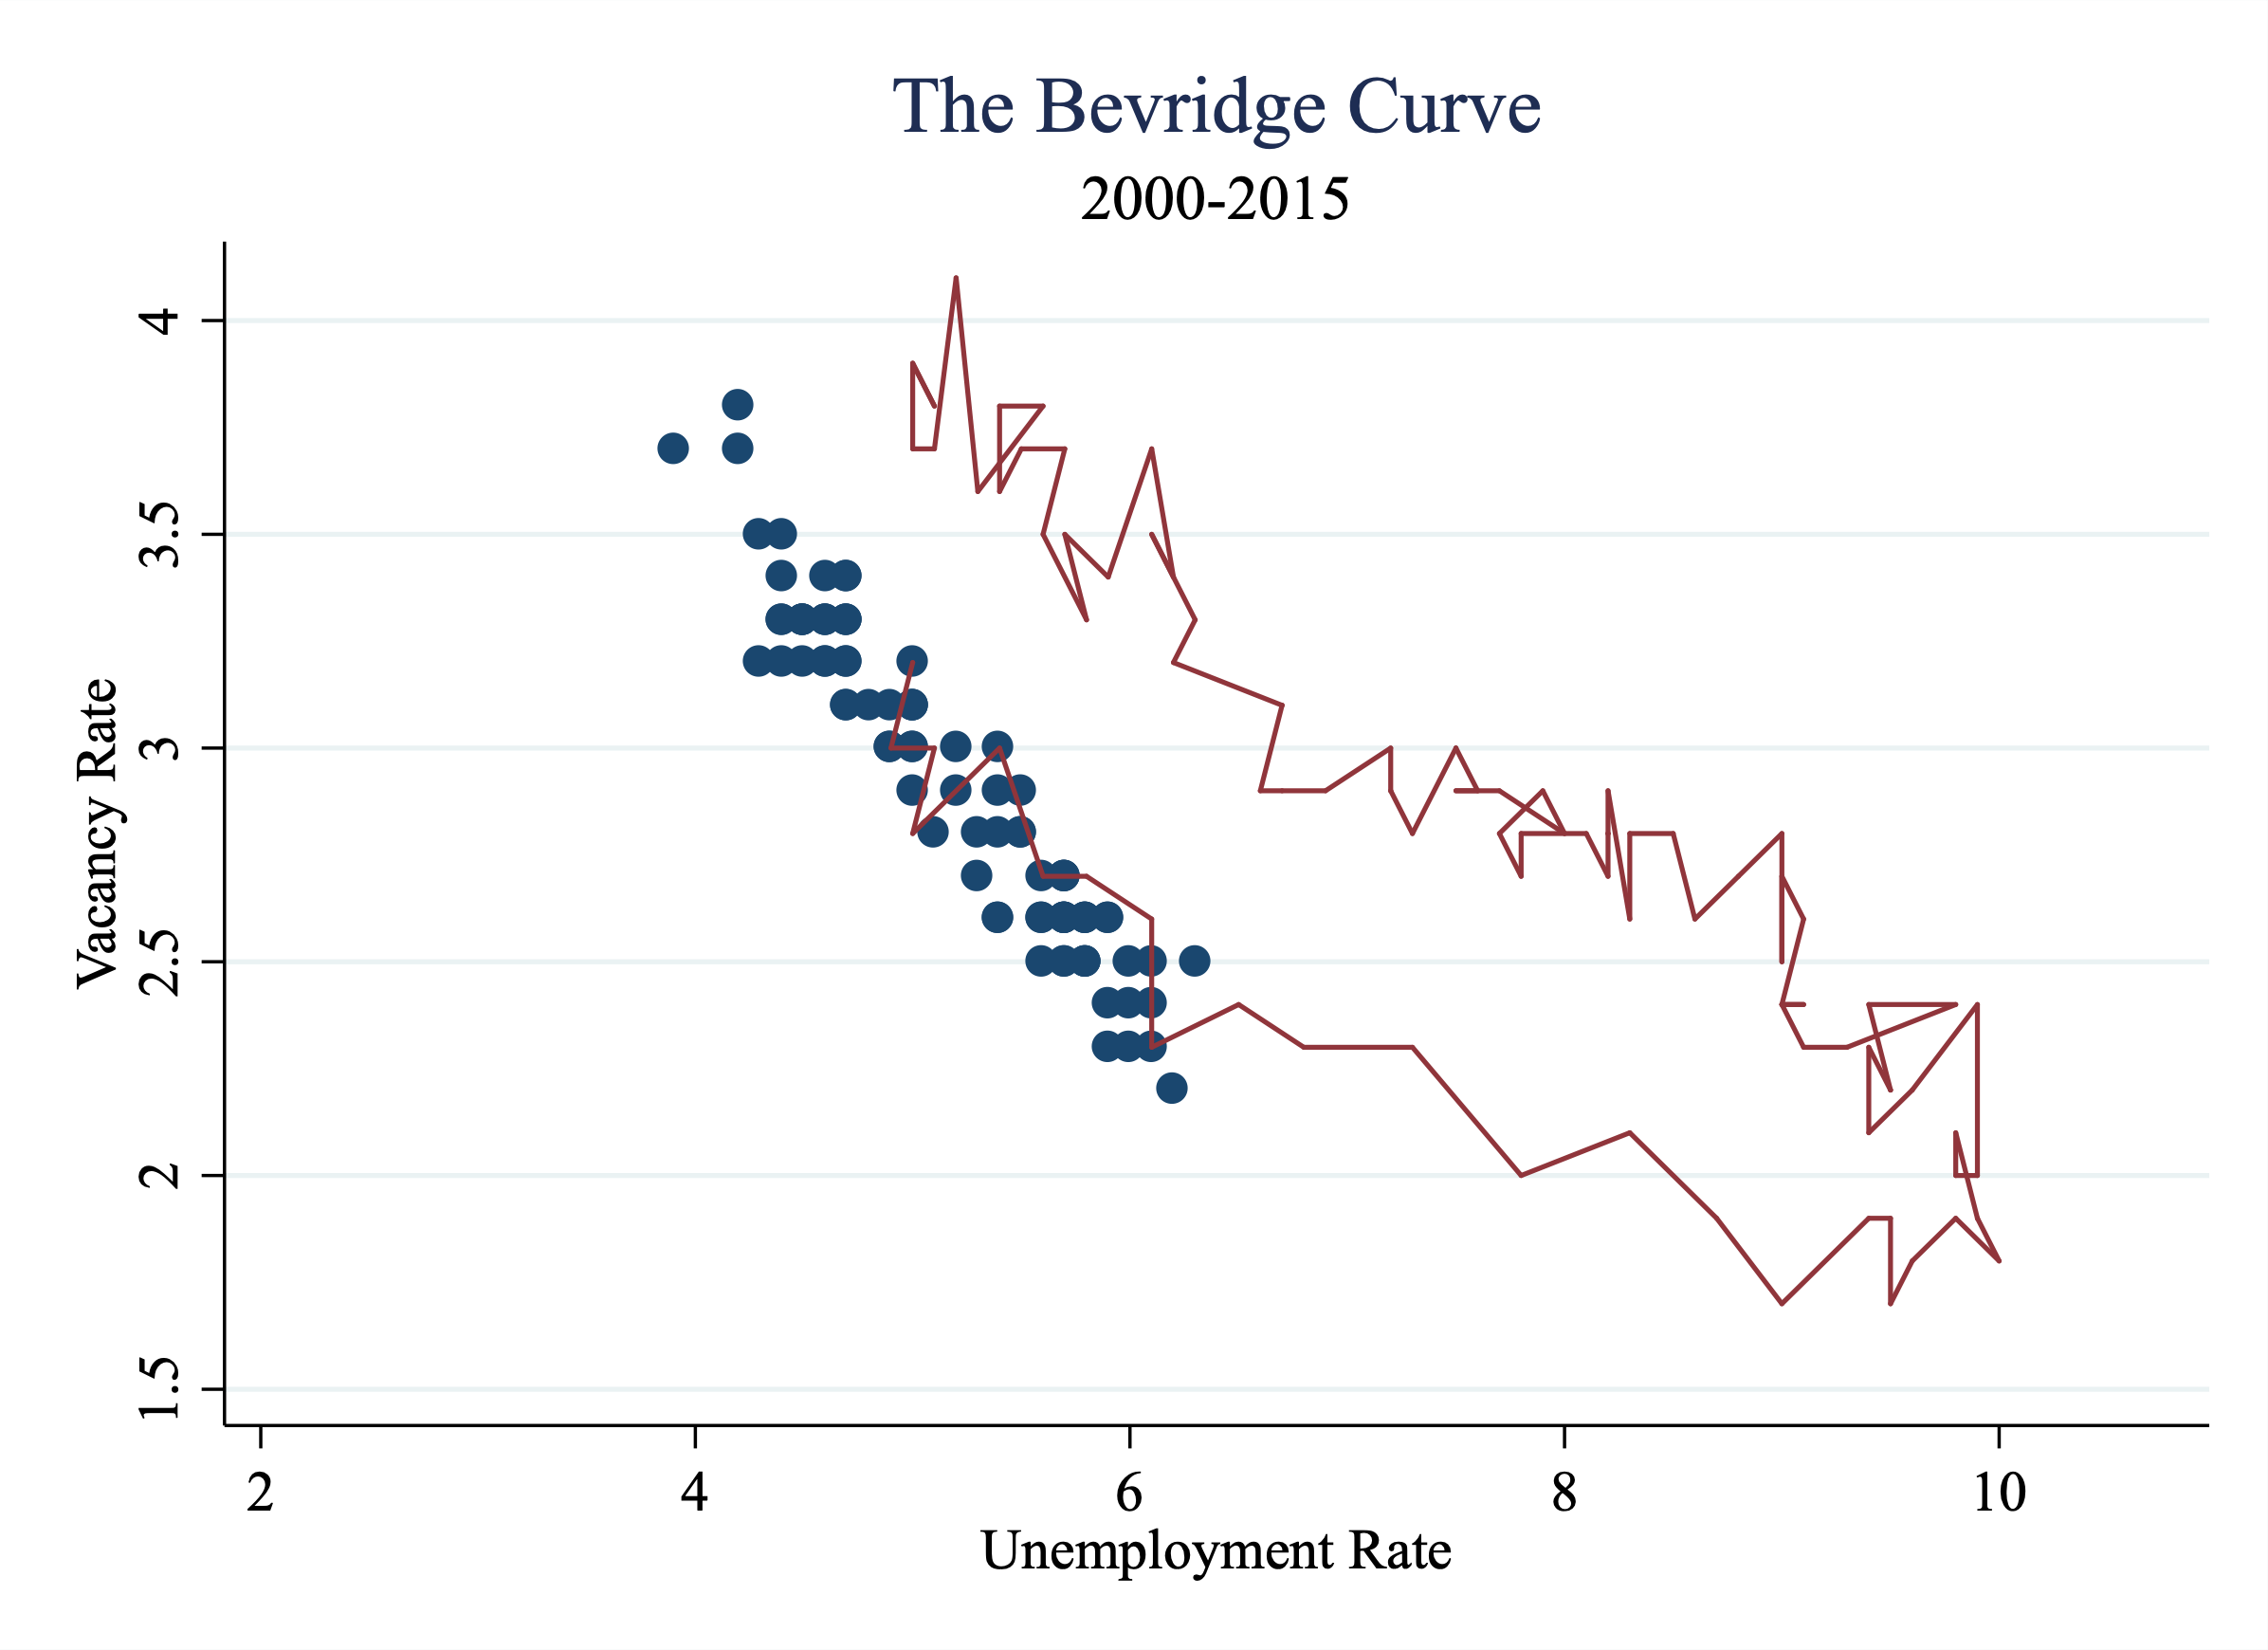
\includegraphics[scale=0.23]{Figures/Fig_6pt8.png}
\end{figure}
hmm...
\end{frame}


\begin{frame}
\frametitle[alignment=center]{Vacancy Rate and the Unemployment Rate}
\begin{figure}
\centering
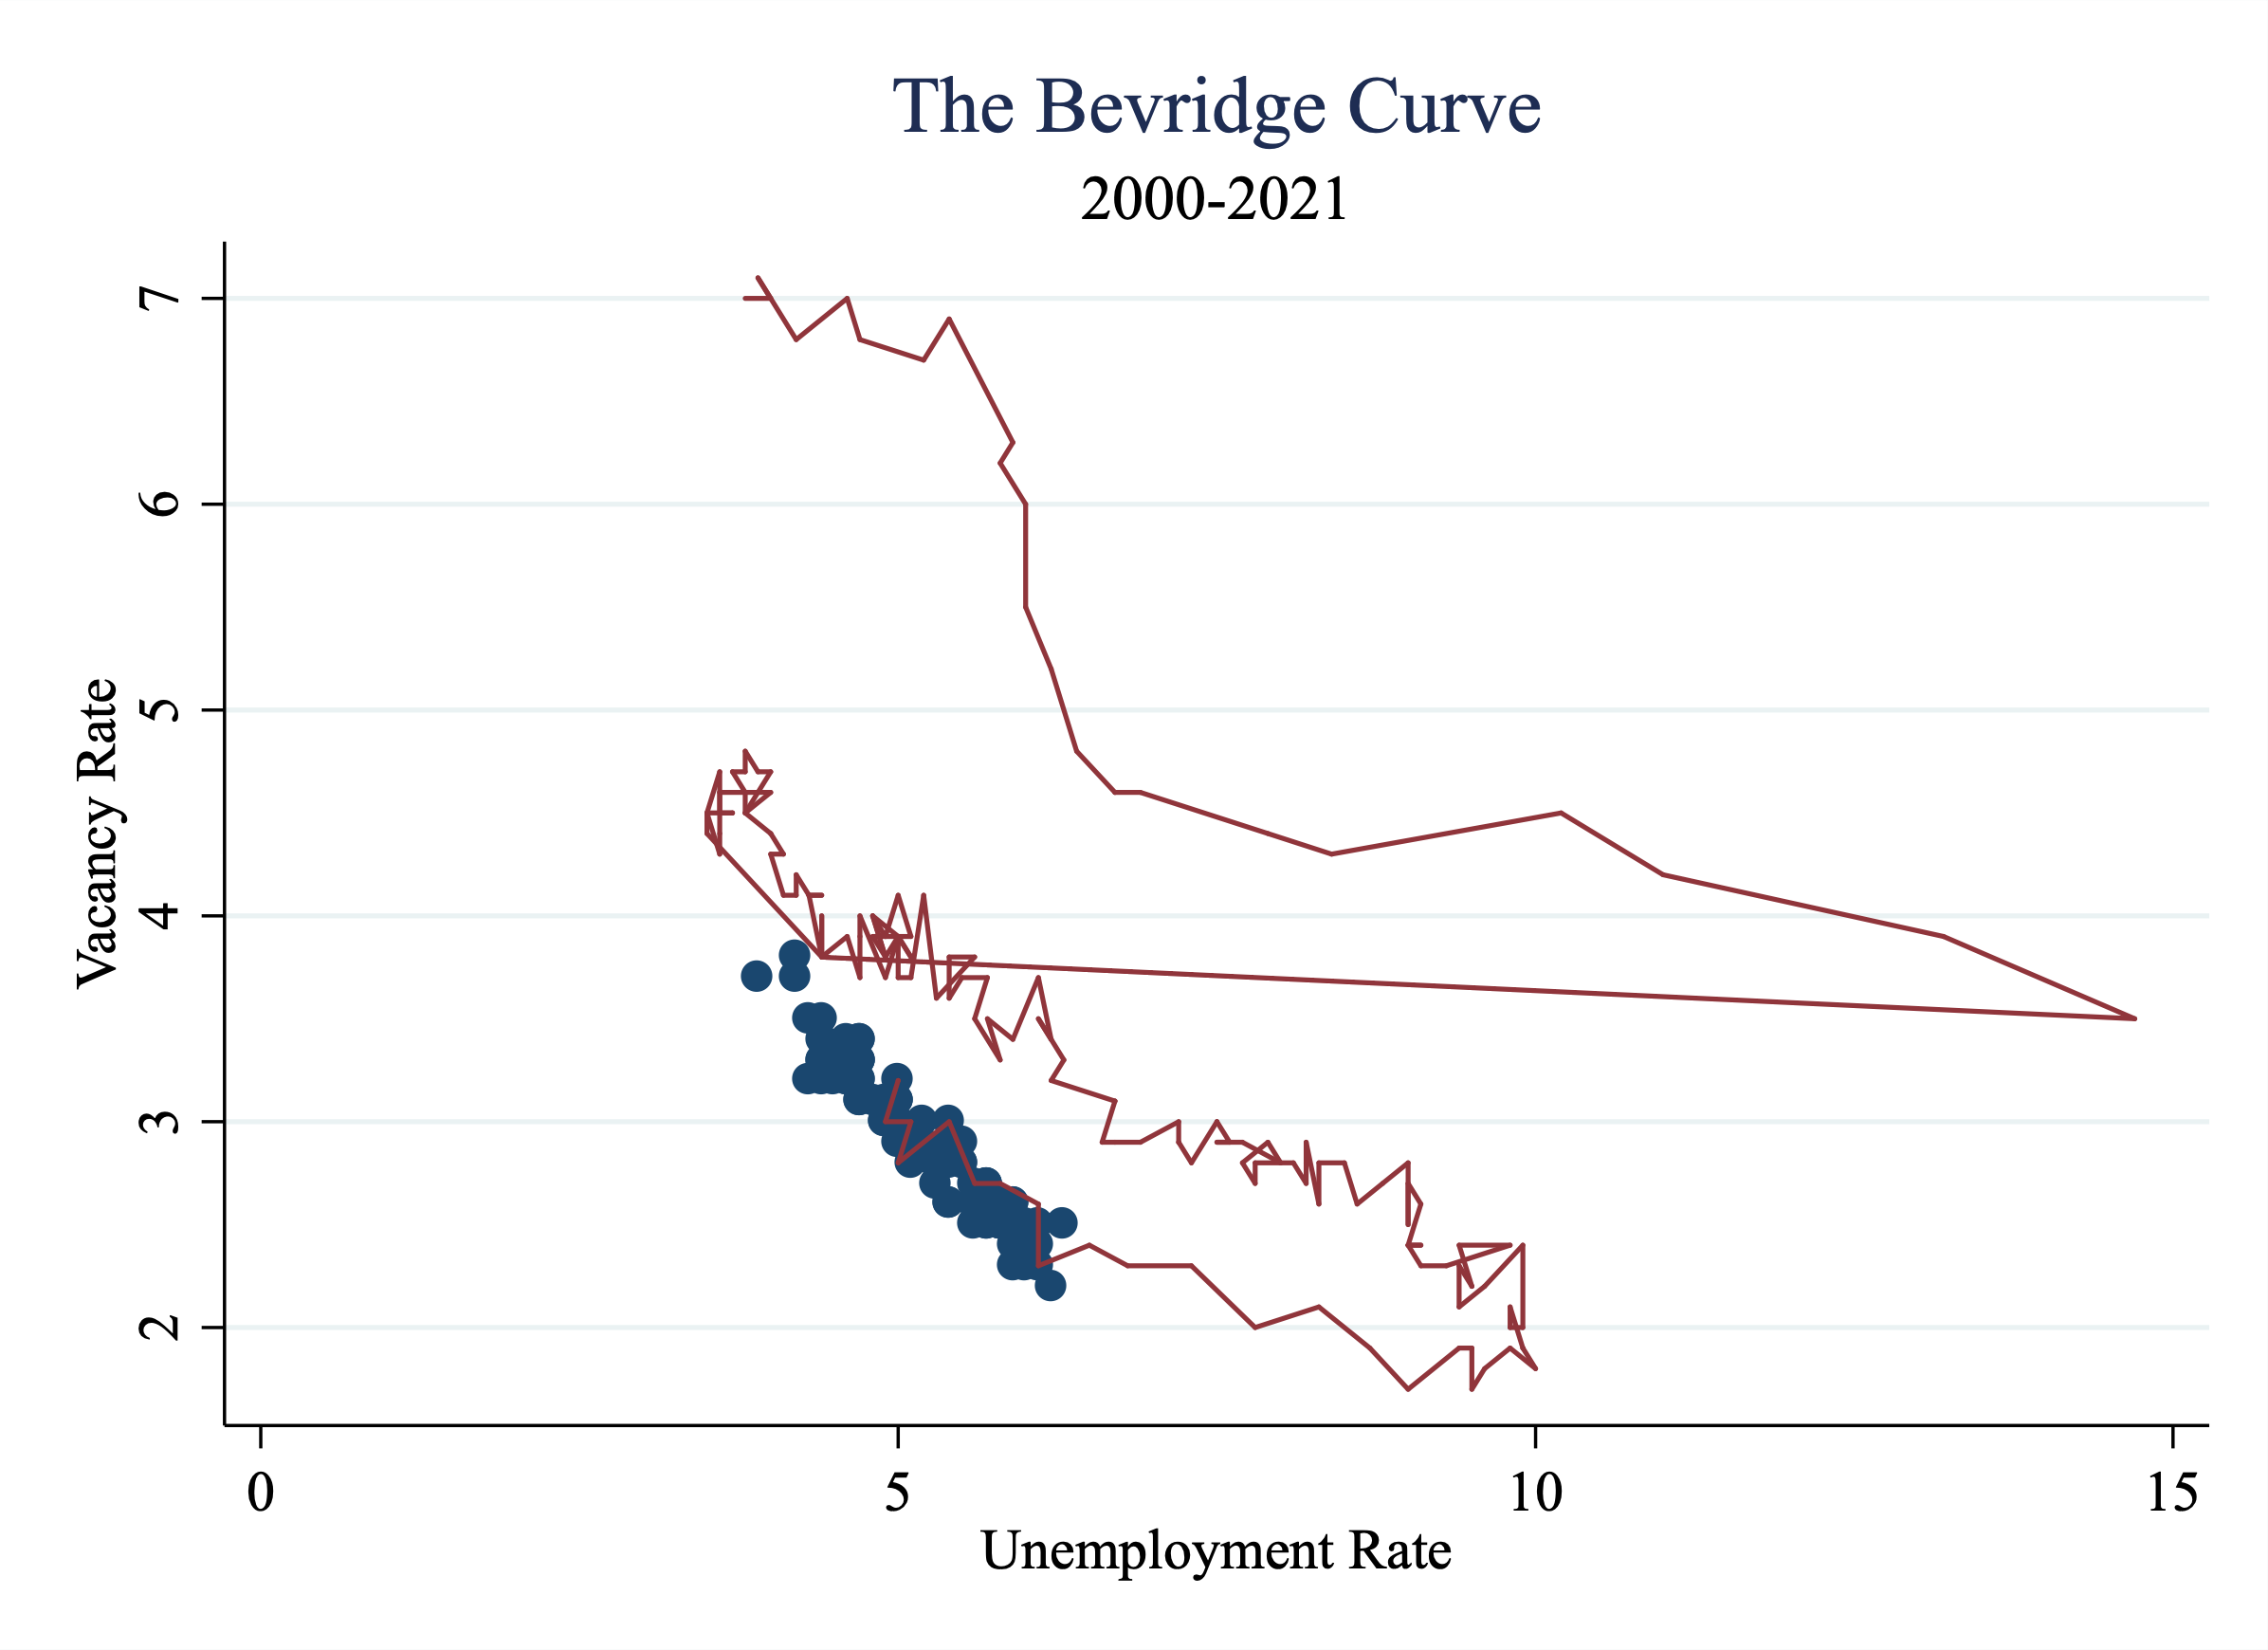
\includegraphics[scale=0.23]{Figures/Fig_6pt8_Updated.png}
\end{figure}
Ah.
\end{frame}

\begin{frame}
\frametitle[alignment=center]{Vacancy Rate and the Unemployment Rate}
\begin{figure}
\centering
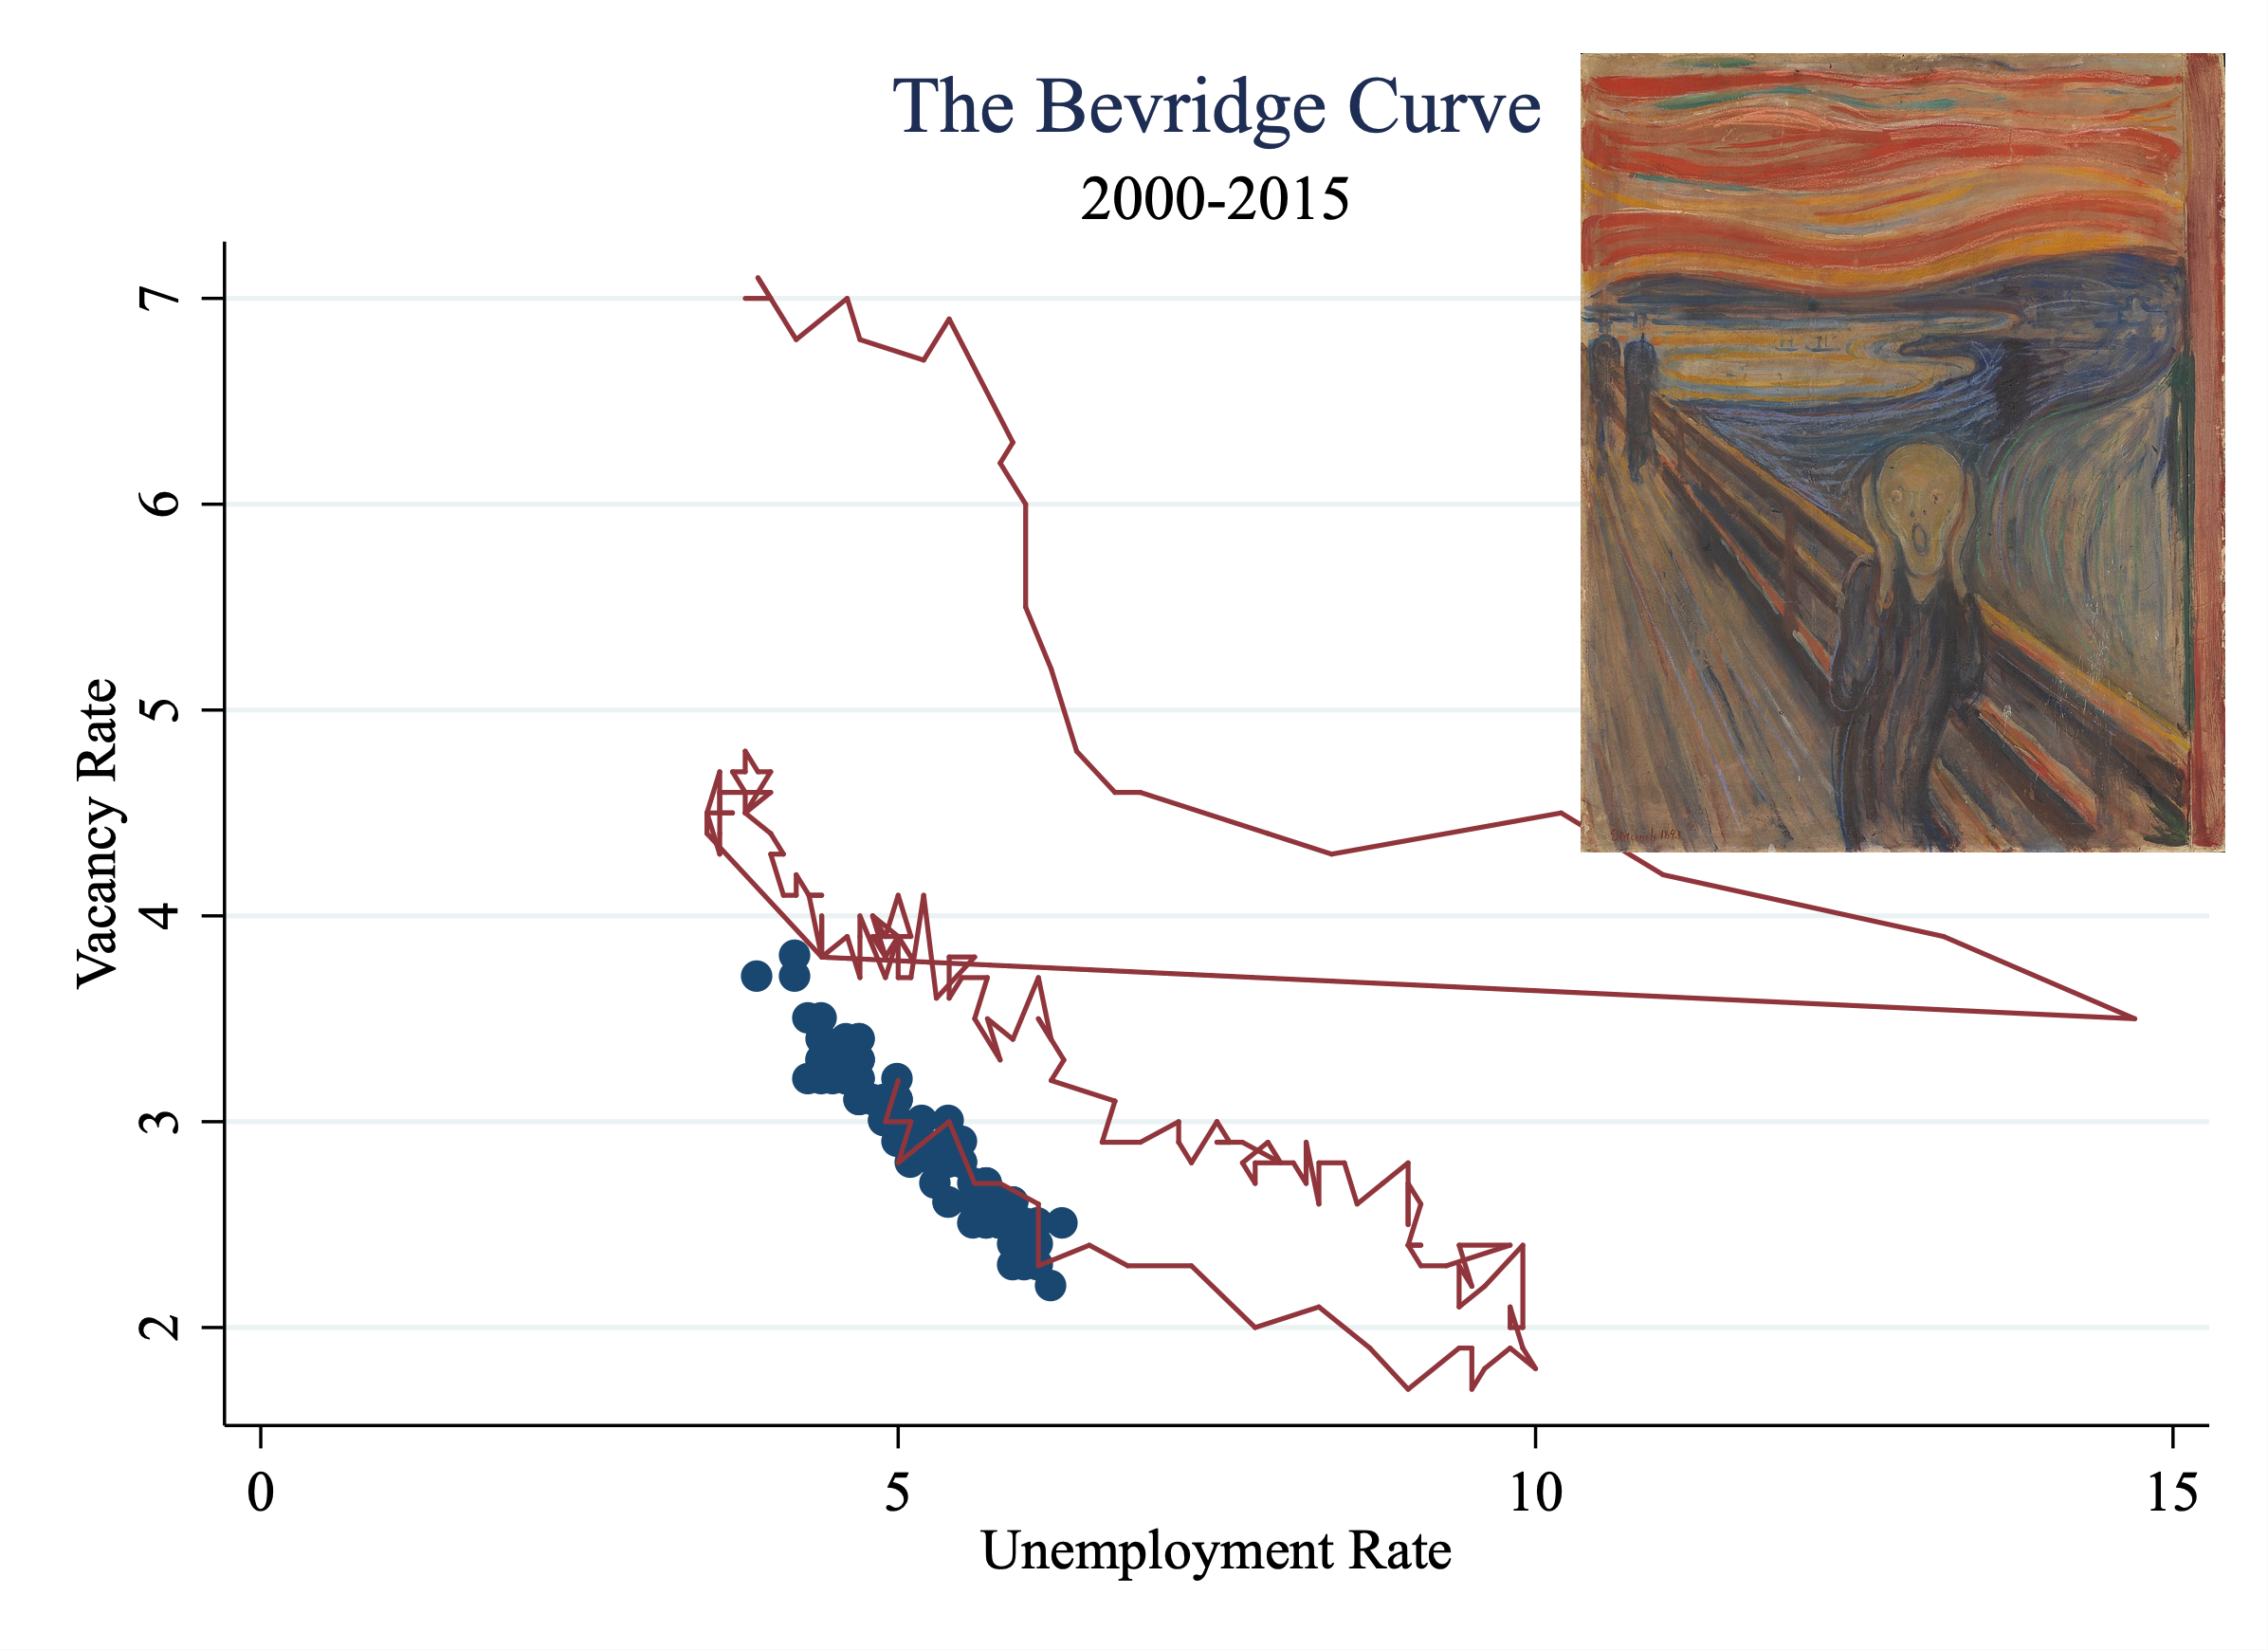
\includegraphics[scale=0.25]{Figures/Fig_6pt8_Updated_Scream.png}
\end{figure}
\end{frame}

\begin{frame}
\frametitle[alignment=center]{One-Sided Search Model of Unemployment}
\begin{itemize}
\item We're going to focus on a worker, who is searching for work and receives job offers that pay particular wages, decides whether or not to accept a job and stop searching ``McCall Search model"
\bigskip
\item We want to understand why people might be unemployed, and search behavior
\bigskip
\item Model:  all workers are in labor force, either employed or unemployed
\bigskip
\item Let $V_e(w)$ denote the value of being employed at wage $w$.  
\item Let $s$ be the probability of losing one's job
\item Let $V_u$ denote the value of being unemployed
\item Let $p$ be the probability of getting a job offer
\item Let's make some predictions about $V_e(w)$ and $V_u$
\end{itemize}
\end{frame}

\begin{frame}
\frametitle[alignment=center]{Predictions}
\begin{itemize}
\item $V_e(w)$ slopes up in the wage ($\frac{\partial V_e(w)}{\partial w}<0$)
\smallskip
\item $V_e(w)$'s slope becomes less positive as wage increases ($\frac{\partial^2 V_e(w)}{\partial w^2}<0$)
\smallskip
\item $V_e(w)$ shifts down when $s$ increases
\smallskip
\item $V_u$  is increasing in unemployment insurance benefits (+value of leisure) $(b)$
\smallskip
\item $V_u$ is increasing in $p$ 
\smallskip
\item The $w$ for which $V_e(w)=V_u$ is called \textbf{the reservation wage} $w^*$:
\begin{itemize}
\item If offered wage is $w\geq w^*$, then accept offer
\item If offered wage is $w<w^*$ then reject
\end{itemize}
\item Let's graph
\end{itemize}
\end{frame}

\begin{frame}
\frametitle[alignment=center]{Welfare of Employed Worker $V_e(w)$}
\begin{figure}
\centering
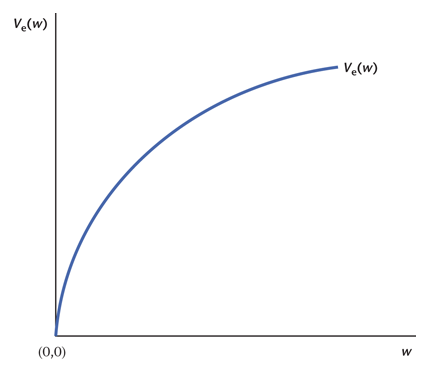
\includegraphics[scale=0.5]{Figures/W_Fig_6pt9.png}
\end{figure}
\end{frame}

\begin{frame}
\frametitle[alignment=center]{Reservation Wage: $V_e(w^*)=V_u$}
\begin{figure}
\centering
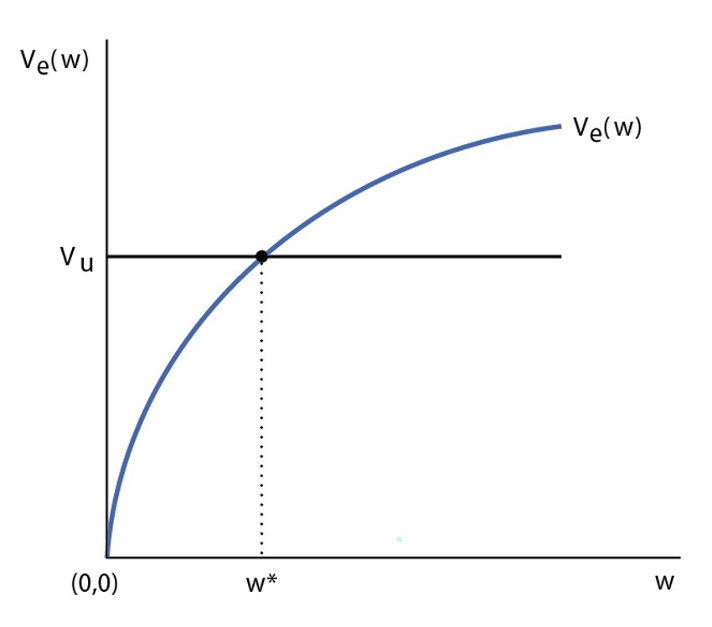
\includegraphics[scale=0.5]{Figures/W_Fig_6pt10.png}
\end{figure}
What happens if we shift the unemployment insurance benefit?
\end{frame}

\begin{frame}
\frametitle[alignment=center]{Increase the unemployment insurance benefit $b$}
\begin{figure}
\centering
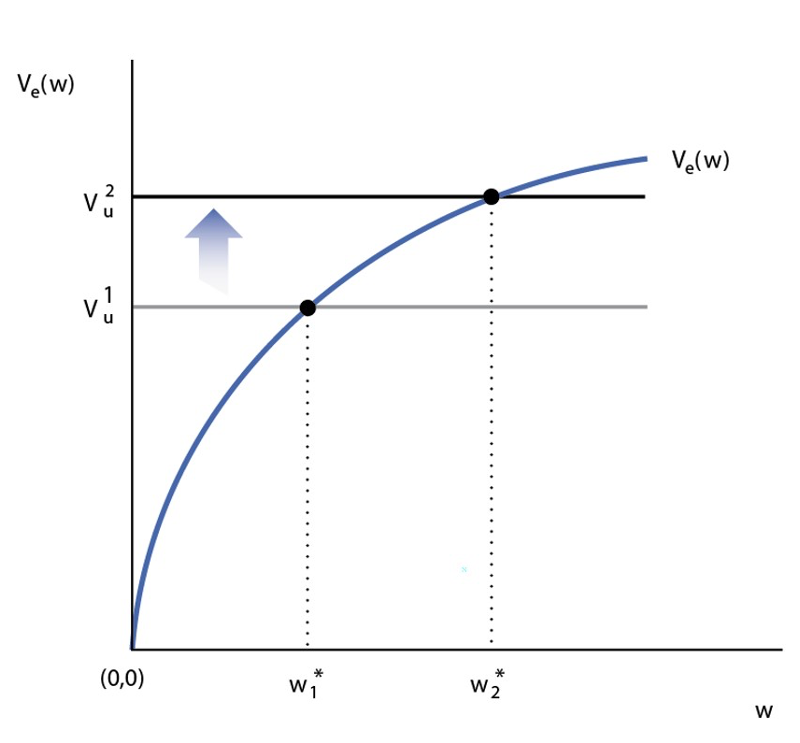
\includegraphics[scale=0.5]{Figures/W_Fig_6pt11.png}
\end{figure}
When $b$ increases, $V_u$ increases, so reservation wage $w^*$ increases
\end{frame}


\begin{frame}
\frametitle[alignment=center]{Determining the Equilibrium Unemployment Rate}
\begin{itemize}
\item Let $U$ be the unemployment rate, $1-U$ be employment rate, and $s$ be the separation rate (emp$\rightarrow$ unemp). 
\bigskip
\item  Then flow into unemployment is $s\cdot (1-U)$
\bigskip
\item Let $H(w^*)$ be the fraction of unemployed workers who that (a) received a wage offer (w/prob $p$), and also had a wage offer greater than $w^*$ 
\bigskip
\item Then $pH(w^*)U$ is the flow into employment (unemp$\rightarrow$ emp)
\bigskip
\item Equilibrium occurs when these two are equal (flows into employment are the same as flows out of unemployment)
$$s(1-U)=pUH(w^*$$
\end{itemize}
\end{frame}

\begin{frame}
\frametitle[alignment=center]{Distribution of Wage Offers Above Threshold}
\begin{figure}
\centering
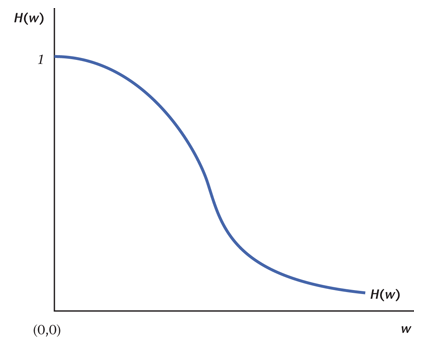
\includegraphics[scale=0.5]{Figures/W_Fig_6pt12.png}
\end{figure}
Idea:  the higher the reservation wage, the smaller the fraction of workers getting that offer (this is just the ``tail distribution" or 1-the CDF of wage offers)
\end{frame}

\begin{frame}
\frametitle[alignment=center]{The Determinants of the Unemployment Rate $U^*$ in the One-Sided Search Model}
\begin{figure}
\centering
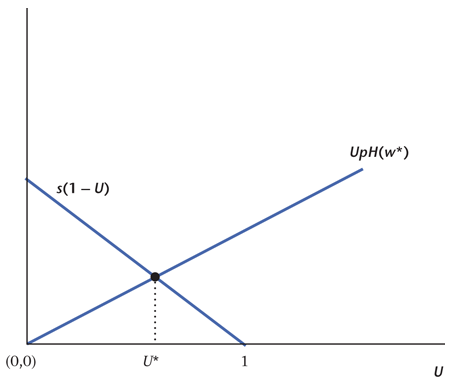
\includegraphics[scale=0.5]{Figures/W_Fig_6pt13.png}
\end{figure}
When $b$ increases, $V_u$ increases, so reservation wage $w^*$ increases
\end{frame}


\begin{frame}
\frametitle[alignment=center]{The Determination of the Reservation Wage and the Unemployment Rate in the One-Sided Search Model}
\begin{figure}
\centering
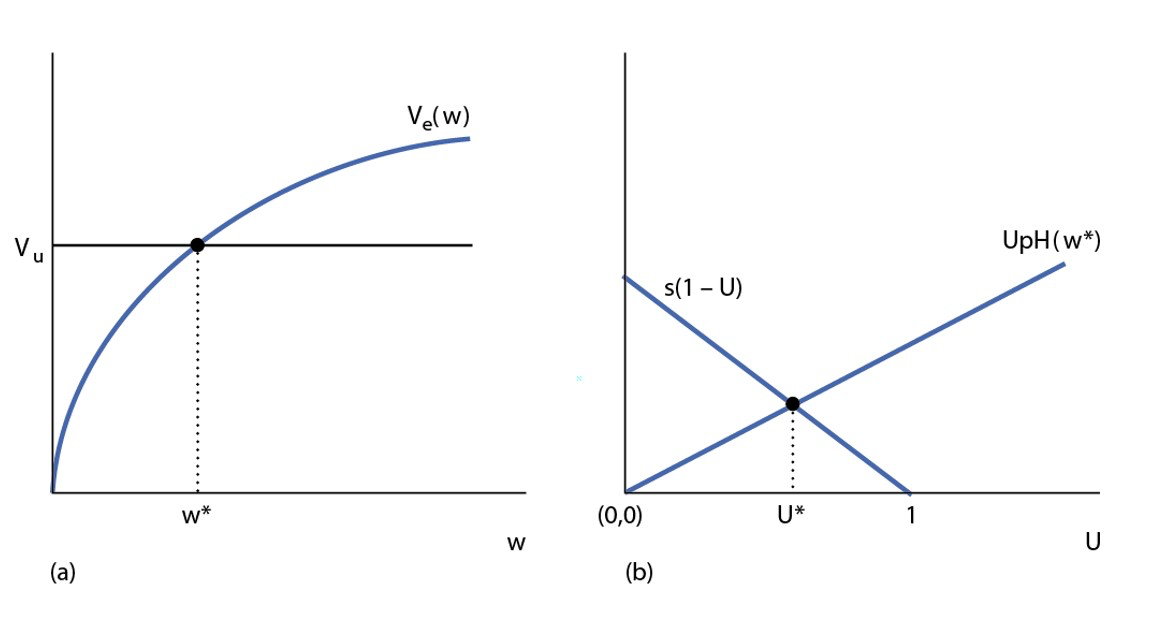
\includegraphics[scale=0.5]{Figures/W_Fig_6pt14.png}
\end{figure}
Putting both our previous figures together.  Now let's use this to analyze increases in $b$ and $p$.
\end{frame}

\begin{frame}
\frametitle[alignment=center]{Increase in Unemployment Insurance Benefits}
\begin{figure}
\centering
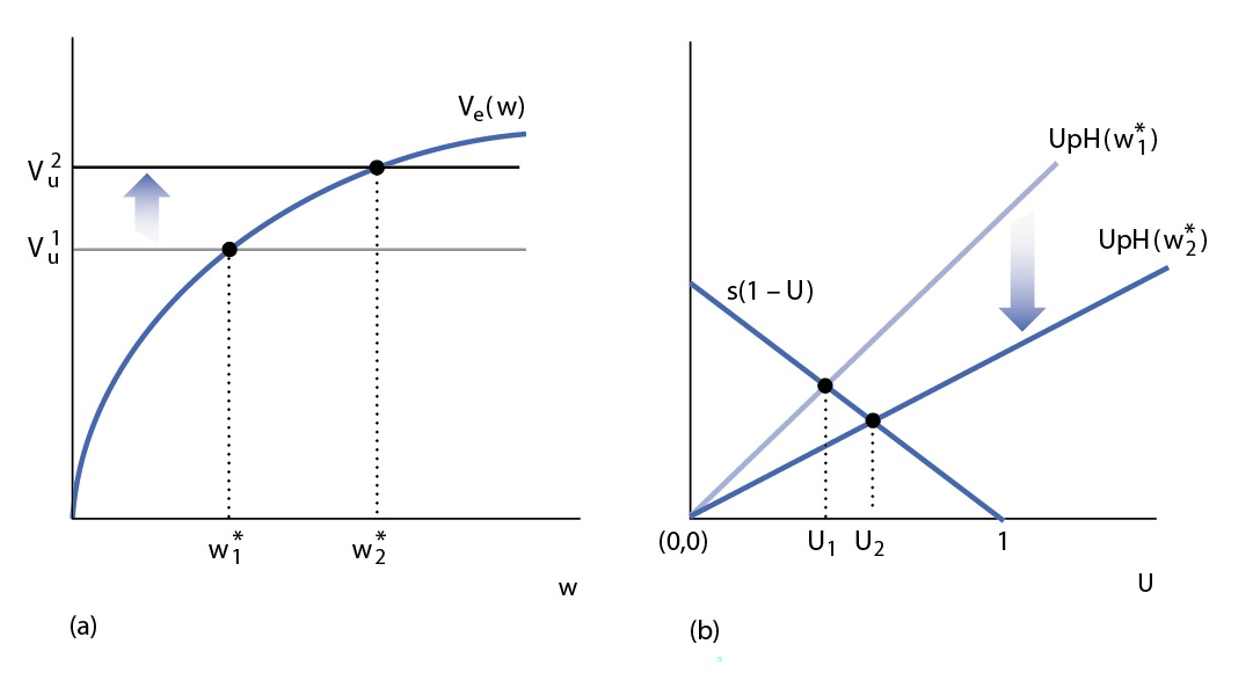
\includegraphics[scale=0.5]{Figures/W_Fig_6pt15.png}
\end{figure}
\end{frame}

\begin{frame}
\frametitle[alignment=center]{Increase in Job Offer Rate}
\begin{figure}
\centering
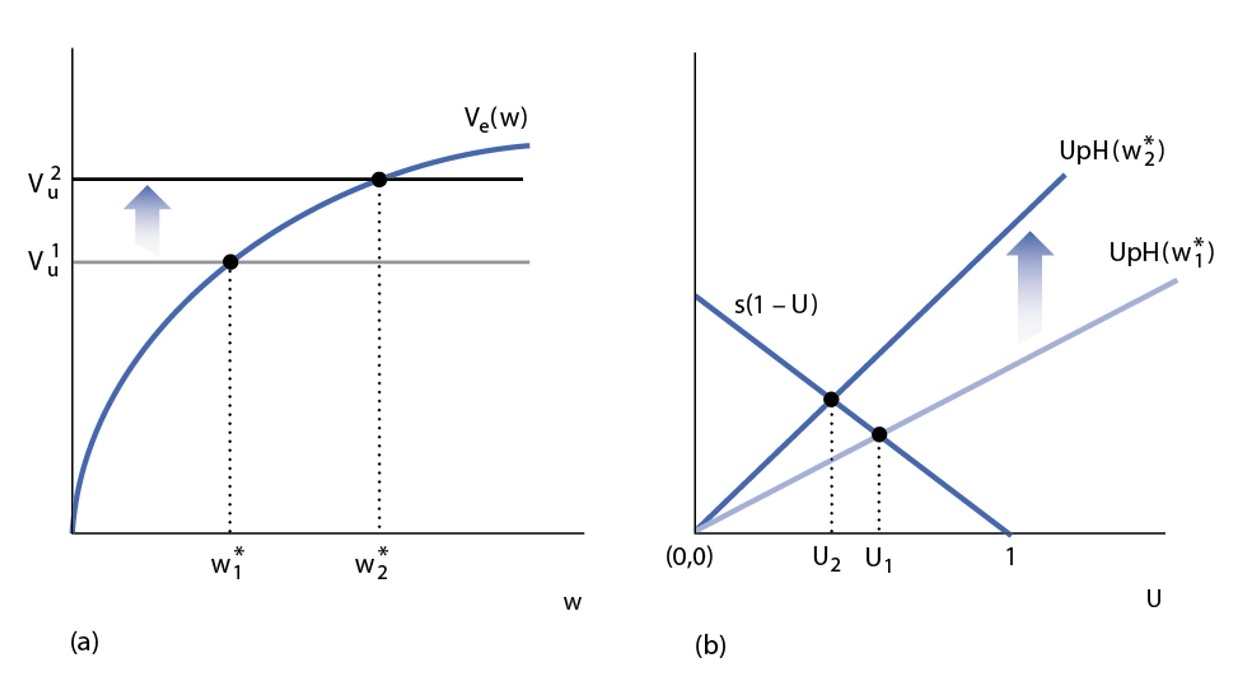
\includegraphics[scale=0.5]{Figures/W_Fig_6pt16.png}
\end{figure}
\end{frame}

\begin{frame}
\frametitle[alignment=center]{Two-Sided Search}
\begin{itemize}
\item This is cool beans and all, but what about the demand side of labor?  Where does $H(w)$ come from?  
\bigskip
\item Let's write down a two-sided model in which workers search for firms and firms search for workers
\end{itemize}
\end{frame}

\begin{frame}
\frametitle[alignment=center]{Two-Sided Search-Setup}
\begin{itemize}
\item Consumers
\begin{itemize}
\item There are $N$ consumers who can either work outside (home production or leisure) the market or search for market work
\bigskip
\item $\mathcal{Q}$ is the quantity of consumers who look for work (labor force) so $N-\mathcal{Q}$ is the quantity who are out of the labor force
\bigskip
\item $P(\mathcal{Q})$ is the supply curve of workers who choose to work for market work: as the wage rises, we expect more workers to look for work
\end{itemize}  
\item Firms
\begin{itemize}
\item It costs firms $k$ (in units of consumption goods) to post a vacancy.  If you don't hire, you shut down (this is a one-period model).  $A$ will denote the number of active firms (number that post vacancies)
\end{itemize}  
\item Environment:
\begin{itemize}
\item When $\mathcal{Q}$ workers search and $A$ firms have vacancies, then the number of matches is determined by the ``matching function" $m$ with efficiency $e$:
$$M=e\cdot m(\mathcal{Q},A)$$
\end{itemize}
\end{itemize}
\end{frame}

\begin{frame}
\frametitle[alignment=center]{Matching Function}
 The matching function is a catch-all that describes how searching workers and firms meet.  We assume that:
 \bigskip
 \begin{enumerate}
\item The matching function is CRS $e\cdot m(x\mathcal{Q},xA)=xe\cdot m(\mathcal{Q},A)$
 \bigskip
\item If no workers search, no matches are made $e\cdot m(0,A)=0$
 \bigskip
\item If no firms have vacancies, no matches are made $e\cdot m(\mathcal{Q},0)=0$
 \bigskip
\item $m$ is increasing in both $\mathcal{Q}$ and $A$
 \bigskip
\item Marginal products are diminishing (increase $\mathcal{Q}$ and hold $A$ constant, and the increase in matches slows
\end{enumerate}
\end{frame}

\begin{frame}
\frametitle[alignment=center]{Supply Side of the Labor Market}
\begin{itemize}
\item This looks a lot like the one-sided market, but now depends on the matching function, rather than an exogenous matching probability $p$
\bigskip
\item Probability a consumer finds a job: $p_c=\frac{e\cdot m(\mathcal{Q},A)}{\mathcal{Q}}$
\bigskip
\item Using constant returns to divide by $\mathcal{Q}$:
$$p_c=m(1,j)$$
\item Where $j=\frac{A}{\mathcal{Q}}$ is the ``market tightness"
\bigskip
\item This is useful:  the probability of finding a job is dependent only on a single parameter $j$!
\bigskip
\item Probability of staying unemployed is now $1-p_c=1-e\cdot m(1,j)$
\bigskip
\item So, supply curve of workers:
$$P(\mathcal{Q})=p_cw+(1-p_c)b=b+e\cdot m(1,j)(w-b)$$
\end{itemize}
\end{frame}
 
\begin{frame}
\frametitle[alignment=center]{Supply Side of the Labor Market}
\begin{figure}
\centering
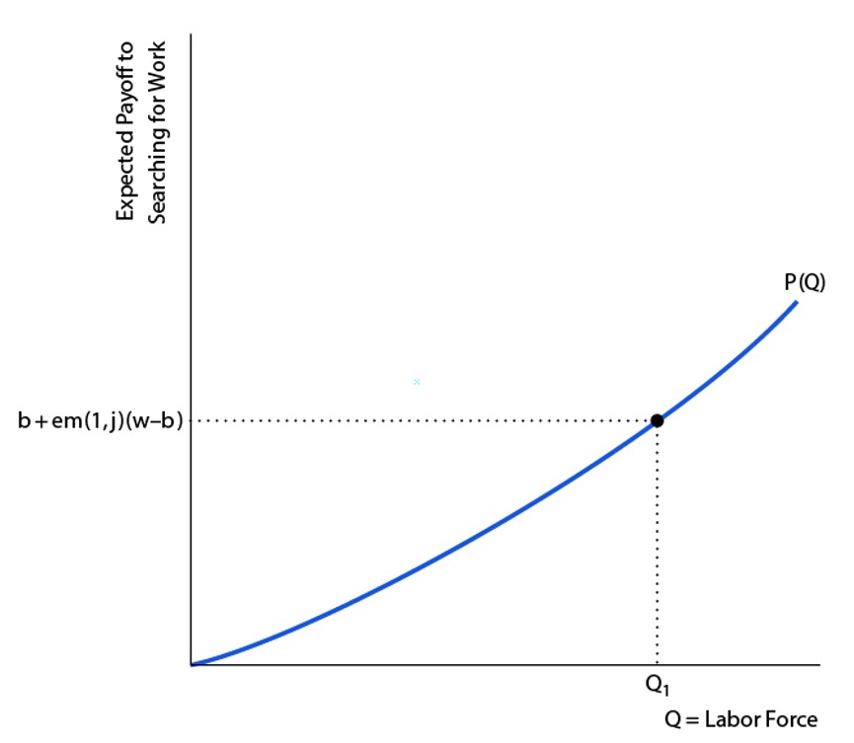
\includegraphics[scale=0.5]{Figures/W_Fig_6pt18.png}
\end{figure}
Market wage, UI benefit, and labor market tightness determine the expected payoff to search, which gives the supply curve of search
\end{frame}

\begin{frame}
\frametitle[alignment=center]{Demand Side of the Labor Market}
\begin{itemize}
\item Now we'll turn to the demand side, which will look similar, but will be simpler
\item Probability a firm finds a worker: $p_f=\frac{e\cdot m(\mathcal{Q},A)}{A}=e\cdot m(\frac{1}{j},1)$ using the same trick as before
\item If a firm matches with a worker, they get $z$, but pay $w$, so on net keep $z-w$, but also pay the vacancy cost $k$ no matter what
\item If firms are free to enter the market, it must be that $\underbrace{p_f}_{\text{pr match}}\underbrace{(z-w)}_{\textbf{payoff if match}}\underbrace{-k}_{\text{vacancy cost}}=0$, the expected payoff is zero 
$$p_c=m(1,j)$$
\item Where $j=\frac{A}{\mathcal{Q}}$ is the ``market tightness"
\item Putting these two together we get:
$$e\cdot m\left(\frac{1}{j},1\right)=\frac{k}{z-w}$$
\item Firms will post vacancies until this is true
\end{itemize}
\end{frame}

 
\begin{frame}
\frametitle[alignment=center]{Demand Side of the Labor Market}
\begin{figure}
\centering
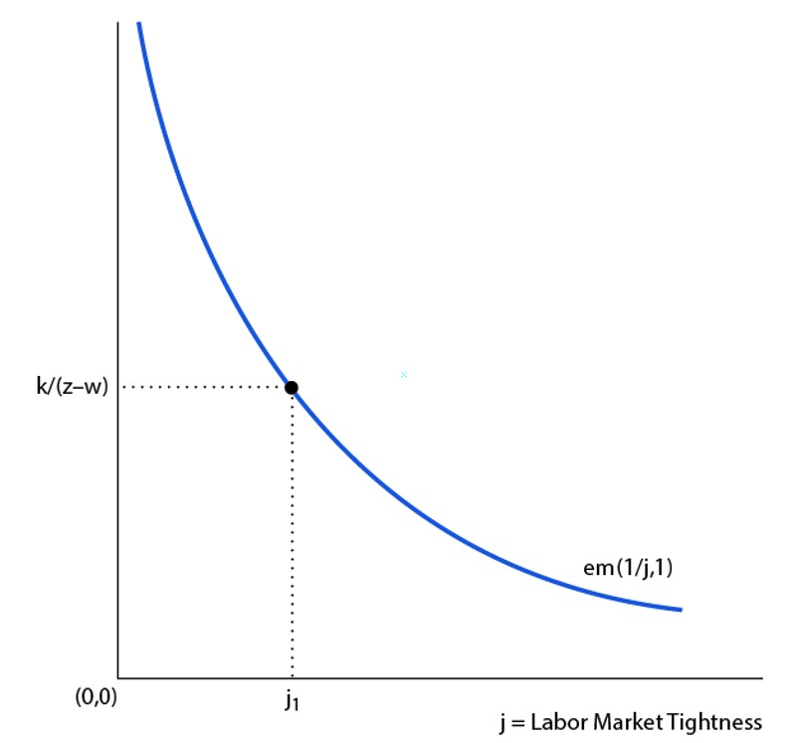
\includegraphics[scale=0.5]{Figures/W_Fig_6pt19.png}
\end{figure}
Firms post vacancies until the probability of matching with a worker is equal to $k/(z-w)$
\end{frame}

 
\begin{frame}
\frametitle[alignment=center]{How is the wage determined?}
\begin{itemize}
\item When a firm matches with a worker, they produce $z$
\item How is $w$ determined?  Who gets the surplus from the match?
\begin{itemize}
\item (This may also inform your understanding of seemingly dysfunctional relationship dynamics!) 
\end{itemize}
\item Could be anything many rules.  One Economists like is ``Nash bargaining theory"
\item Think about the options of each party:
\begin{itemize}
\item Worker's next best option is $b$, so surplus is $w-b$
\item Firm's next best option is 0 ($k$ is lost no matter what) so surplus is $z-w$
\item Worker+firm surplus is $z-b$
\end{itemize}
\item Nash bargaining predicts/dictates that each gets a constant share of total surplus.  $a$ will be the worker's share:
$$w-b=a(z-b)$$
\item Solving for the wage:
$$w=az+(1-a)b$$
\end{itemize}
\end{frame}

 
\begin{frame}
\frametitle[alignment=center]{How is the wage determined?}
\begin{itemize}
\item Nash bargaining wage:
$$w=az+(1-a)b$$
\item Substituting into the supply and demand curves for labor we derived earlier:
$$P(\mathcal{Q})=b+e\cdot m(1,j)a(z-b)$$
$$e\cdot m\left(\frac{1}{j},1\right)=\frac{k}{(1-a)(z-b)}$$
\item $j$ will be determined by the second equation, which then determines $\mathcal{Q}$ in the first
\end{itemize}
\end{frame}

\begin{frame}
\frametitle[alignment=center]{Equilibrium in the Two-Sided Search Model}
\begin{figure}
\centering
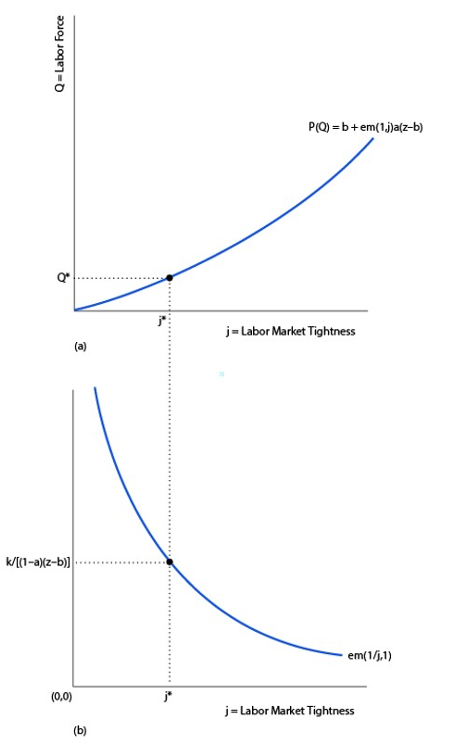
\includegraphics[scale=0.5]{Figures/W_Fig_6pt20.png}
\end{figure}
Demand side determines $j^*$, which then determines $\mathcal{Q}^*$
\end{frame}

\begin{frame}
\frametitle[alignment=center]{Equilibrium in the Two-Sided Search Model-Continued}
\begin{itemize}
\item With market tightness $j^*$ and labor force $\mathcal{Q}$, can determine
\bigskip
\item With $\mathcal{Q}$ we also know not in labor force $N-\mathcal{Q}$, and the unemployment rate:
$$U=\frac{\mathcal{Q}(1-p_c)}{\mathcal{Q}}=1-e\cdot m(1,j)$$
\item We also have the vacancy rate:
$$v=\frac{A(1-p_f)}{A}=1-e\cdot m\left(\frac{1}{j},1\right)$$
\item The total output in the economy is the number of matches $M$ times productivity:
$$Y=Mz$$ 
\item Or:
$$Y=e\cdot m(\mathcal{Q},A)z=\mathcal{Q}e\cdot m(1,j)z$$
\item Now let's apply it
\end{itemize}
\end{frame}


\begin{frame}
\frametitle[alignment=center]{Two-Sided Model:  Increasing the UI Benefit}
\begin{itemize}
\item When the UI benefit $b$ increases, the worker's outside option increases.  But the wage is given by:
$$w=az+(1-a)b$$
\item So workers wages increase
\bigskip
\item Firm surplus $z-w$ falls, but it's still the case that:
$$e\cdot m\left(\frac{1}{j},1\right)=\frac{k}{z-w}$$
\item Fixing vacancy cost $k$ and productivity $z$, it must be that when the RHS rises, market tightness $j$ must fall so the LHS rises commensurately
\bigskip
\item In lay terms:  firms now get less from each match, so the probability of matching must rise to make up for their loss (if it didn't, they would make negative profits, so firms leave until they make zero again)
\end{itemize}
\end{frame}


\begin{frame}
\frametitle[alignment=center]{Equilibrium in the Two-Sided Search Model}
\begin{figure}
\centering
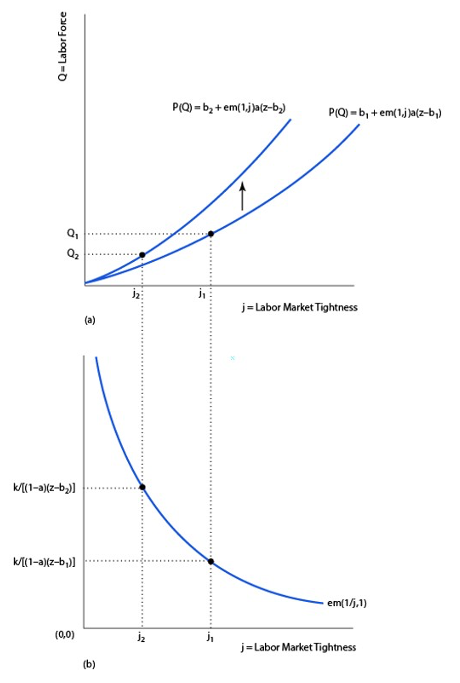
\includegraphics[scale=0.5]{Figures/W_Fig_6pt21.png}
\end{figure}
When $b$ increases, firm search falls, and tightness increases.  Meanwhile, supply shifts out, so that $\mathcal{Q}$ could increase or decrease 
\end{frame}


\begin{frame}
\frametitle[alignment=center]{Two-Sided Model:  Increasing the UI Benefit-Continued}
\begin{itemize}
\item Recall that $P(\mathcal{Q})=b+e\cdot m(1,j)a(z-b)$, so $b$ rises (labor force rises) but $j$ falls (so labor force falls). Ambiguous!
\bigskip
\item But it's certain that $U$ will rise and $v$ will fall:
$$U=1-e\cdot m(1,j)$$
$$v=1-e\cdot m\left(\frac{1}{j},1\right)$$
\item What happens to total output:  $Y=zM$: ambiguous, depends on what happens to $\mathcal{Q}$.
\bigskip
\item In general, higher $b$ has two effects: draws people in to searching for a job (increase GDP) but also pays people not to work (decrease GDP)
\bigskip
\item Theoretically ambigious affect on $Y$, but predicts high $b$ countries should have higher ``labor forces" but also higher unemployment
\end{itemize}
\end{frame}

\begin{frame}
\frametitle[alignment=center]{Equilibrium in the Two-Sided Search Model}
\begin{figure}
\centering
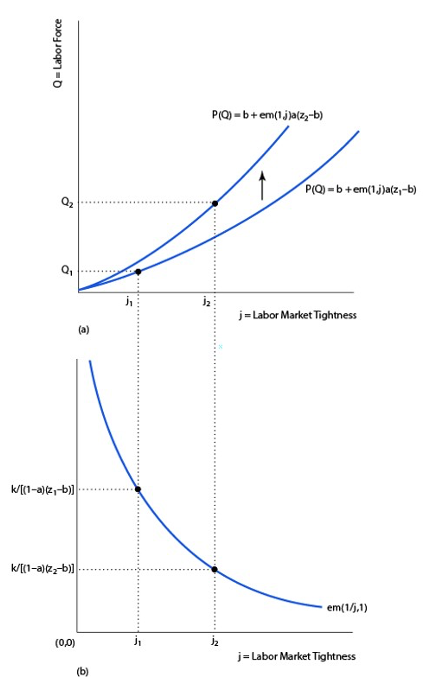
\includegraphics[scale=0.5]{Figures/W_Fig_6pt22.png}
\end{figure}
When $z$ increases, firm search rises, and tightness increases.  Meanwhile, supply shifts out, so that $\mathcal{Q}$ increases unambiguously 
\end{frame}



\begin{frame}
\frametitle[alignment=center]{Two-Sided Model:  Increasing Productivity}
\begin{itemize}
\item Now $z$ increases.  Again, start from wage: 
$$w=az+(1-a)b$$
\item Wage increases by $az$ what about firm side?
$$e\cdot m\left(\frac{1}{j},1\right)=\frac{k}{z-w}$$
\item When $z$ rises, then the RHS falls, so $j$ must rise (labor tightness rise)
\item And labor force (both $j$ rises and $z-b$ rises, so $P(\mathcal{Q})$ definitely rises:
$$P(\mathcal{Q})=b+e\cdot m(1,j)a(z-b)$$
\item Unemployment falls and vacancies rise
$$U=1-e\cdot m(1,j)\ \ \ \ v=1-e\cdot m\left(\frac{1}{j},1\right)$$
\item  $Y=\overbrace{\mathcal{Q}}^{\uparrow}e\cdot \overbrace{m(1,j)}^{\uparrow}\overbrace{z}^{\uparrow}$ increases
\end{itemize}
\end{frame}

\begin{frame}
\frametitle[alignment=center]{Does productivity fit with what we see in the business cycle?}
\begin{itemize}
\item Prediction: when $z$ rises:
\begin{itemize}
\item Labor force $\mathcal{Q}$ increases
\item Employment $\mathcal{Q}-U$ increases
\item Vacancies $v$ increase
\item Wages $w$ increase 
\item Unemployment rate $U$ falls
\item Total production $Y$ increases
\item Concurrent increases in $v$ and decreases in $U$ are what the Beveridge curve shows
\item Good!
\end{itemize}
\item Let's turn to our last application: efficiency of matching rate
\end{itemize}
\end{frame}

\begin{frame}
\frametitle[alignment=center]{Two-Sided Model:  Decrease in Matching Efficiency}
\begin{itemize}
\item Now $e$ decreases.  Again, start from wage: 
$$w=az+(1-a)b$$
\item Wage is unchanged. Firm side?
$$e\cdot m\left(\frac{1}{j},1\right)=\frac{k}{z-w}$$
\item When $e$ falls, then $j$ must fall to keep the LHS the same
\item When $j$ falls, then the supply curve shifts down for two reasons:
$$P(\mathcal{Q})=b+e\cdot m(1,j)a(z-b)$$
\item So $\mathcal{Q}$ falls.  Unemployment rises and vacancies fall
$$U=1-e\cdot m(1,j)\ \ \ \ v=1-e\cdot m\left(\frac{1}{j},1\right)$$
\item  $Y=\mathcal{Q}e\cdot m(1,j)z$ falls
\end{itemize}
\end{frame}


\begin{frame}
\frametitle[alignment=center]{Equilibrium in the Two-Sided Search Model}
\begin{figure}
\centering
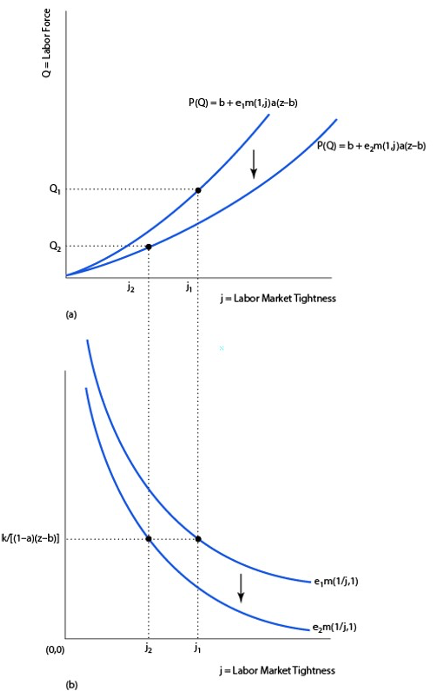
\includegraphics[scale=0.5]{Figures/W_Fig_6pt23.png}
\end{figure}
When $e$ decreases, firm search falls, worker search falls
\end{frame}

\begin{frame}
\frametitle[alignment=center]{Two-Sided Model:  Decrease in Matching Efficiency}
\begin{itemize}
\item Decreases in matching efficiency might happen when we have ``sectoral shocks" and ``mismatch"
\bigskip
\item Suddenly workers and firms are looking for different things
\bigskip
\item Would be a shift \emph{out} in the Beveridge curve
\end{itemize}
\end{frame}

\begin{frame}
\frametitle[alignment=center]{Summary: how to think in the two sided model}
\begin{itemize}
\item We have two simple equations, so start with them:
$$w=az+(1-a)b$$
$$e\cdot m\left(\frac{1}{j},1\right)=\frac{k}{z-w}$$
\item The first gives you how $w$ changes when $z$ or $b$ changes
\item The second gives you how $j$ changes when $e$, $k$, $z$, or $w$ change
\item Once you have how $j$ changes, you can think about the labor supply side:
$$P(\mathcal{Q})=b+e\cdot m(1,j)a(z-b)$$
\item And with that you can figure out unemployment, vacancies, production, etc.
\end{itemize}
\end{frame}

\begin{frame}
\frametitle[alignment=center]{Simple One-Period Models}
\begin{itemize}
\item Now you've seen our simple one-period models (for the market-clearing model and the unemployment/search-and-matching model
\bigskip
\item We'll turn to growth next section
\end{itemize}
\end{frame}





\end{document}